\documentclass{book}
\usepackage[utf8]{inputenc}
\usepackage[spanish]{babel}
\usepackage{csquotes}
\usepackage[backend=bibtex,style=numeric]{biblatex}
\usepackage{dsfont}% Esta pone los contents y las referencias de imagen
\usepackage{graphicx} %Estaaa da error de logreq
\usepackage{amsmath}
\usepackage{mathtools}
\usepackage{amssymb}
\usepackage{color}
\usepackage{subfigure}
\usepackage{float}
\usepackage{capt-of}
\usepackage{sidecap}
\sidecaptionvpos{figure}{c}
\usepackage{caption}
\usepackage{commath}
\usepackage{latexsym, amsfonts, epsfig, enumerate, listings, fancyhdr}
\usepackage{cancel}
\usepackage[table,xcdraw]{xcolor}
\usepackage{cancel}
%\usepackage{anysize} 				
%\marginsize{2cm}{2cm}{2cm}{2cm} % Izquierda, derecha, arriba, abajo
% Para que las referencias sean hipervínculos a las figuras o ecuaciones y
% aparezcan en color
\usepackage[colorlinks=true,plainpages=false,citecolor=blue,linkcolor=blue]{hyperref}
\usepackage{fancyhdr} 
\pagestyle{fancy}
\fancyhf{}
%\fancyhead[L]{\footnotesize Universidad Nacional Autónoma de México} %encabezado izquierda
\fancyfoot[C]{\thepage}  %centro
\renewcommand{\footrulewidth}{0.4pt}
\usepackage{listings}
\bibliography{Referencias}

\begin{document}
\begin{center}
\thispagestyle{empty}				
\newcommand{\HRule}{\rule{\linewidth}{0.5mm}}
\pagenumbering{Roman}
\begin{minipage}{\textwidth} \begin{center}

\includegraphics[scale = 0.3]{Figures/UNAM_blue.png}
\end{center}\end{minipage}
\vspace*{1cm}\\
\textbf{\textsc{\large UNIVERSIDAD NACIONAL AUTÓNOMA DE MÉXICO}}\\[0.3cm]

\textsc{PROGRAMA DE MAESTRÍA Y DOCTORADO EN INGENIERÍA}\\[0.3cm]

\textsc{ELÉCTRICA - PROCESAMIENTO DIGITAL DE SEÑALES}\\[1cm]
						
\textbf{\textsc{PERCEPCIÓN ARTIFICIAL Y PLANEACIÓN DE ACCIONES A PARTIR DE LA CÁMARA RGBD DE UN ROBOT MÓVIL}}
\\[1cm]

\textsc{TESIS}\\
\vspace*{0.2cm}
\textsc{QUE PARA OPTAR POR EL GRADO DE:}\\
\vspace*{0.2cm}
\textsc{MAESTRA EN INGENIERÍA}\\
\vspace*{1cm}

\textsc{PRESENTA:}\\
\vspace*{0.2cm}
\textsc{MITZI ANAID RAMÍREZ ESTRADA}\\
\vspace*{1.5cm}

\textsc{TUTORES:}\\
\vspace*{0.2cm}
\textsc{DR. JESÚS SAVAGE CARMONA}\\
\vspace*{0.2cm}
\textsc{DR. MARCO ANTONIO NEGRETE VILLANUEVA}\\
\vspace*{0.2cm}
\textsc{FACULTAD DE INGENIERÍA, UNAM}\\
\vspace*{1cm}

\textsc{CIUDAD UNIVERSITARIA, CD. MX. AGOSTO, 2024}
\end{center}
\tableofcontents
\pagenumbering{arabic}
\chapter{Introducción}

Actualmente uno de los temas que se encuentran en apogeo y con mucho reconocimiento de la aplicación de los avances tecnológicos es la robótica. Constantemente se desarrollan nuevas tecnologías que es posible implementar tanto en el software como en el hardware de estas herramientas, además de la paulatina integración de estos elementos en la vida diaria, en entornos y aplicaciones diversas.


No resulta extraño mencionar que el ambiente donde con más frecuencia se encuentran estos elementos es el industrial, donde desde hace varias décadas es posible encontrar centros de producción masiva en que brazos robóticos y bandas transportadoras se encargan del ensamblaje en serie de diferentes productos. Utilizando dicho modelo, donde se encuentran comunicados y \textit{encadenadas} todas las etapas de la producción de los productos, se obtienen fábricas en las que es posible producir una gran cantidad del mismo tipo de producto.


 El anterior es uno de los motivos por los cuales se ha encontrado necesaria la introducción de modelos de producción más flexibles, quizás para plantas menos especializadas o para productos que no requieran ser construidos de forma masiva, haciendo posible utilizar las alas industriales de formas variadas para el ensamblaje de productos variados. Así, considerando que las máquinas que se encargan de las etapas de producción no se encuentren físicamente ligadas unas con otras, aunque sí se encarguen de desempeñar tareas específicas dentro de un proceso secuencial, se obtiene el concepto de fábricas inteligentes, correspondientes a la llamada Industria 4.0, aveces mencionada como la 4ta revolución industrial (\cite{kohout_multi-robot_2020}).

Navarro Piña menciona que el Instituto Norteamericano de Robótica describe el \textbf{robot industrial} como: "\textit{un manipulador multifuncional y programable, diseñado para mover materiales, piezas, herramientas o dispositivos especiales mediante movimientos programados y variables que permiten llevar a cabo diversas tareas (\cite*{navarro_pina_robot_2021})}", siendo estos los antes mencionados brazos armadores que típicamente se ven en las plantas industriales. 

Por otro lado, \cite{basco_industria_2018}, enfatizan la importancia de la robótica colaborativa, en la cual la flexibilidad y versatilidad de las plantas es imperativa, integrando sistemas que puedan sumarse al sistema de producción  mediante el transporte de productos intermedios y finales entre estaciones de trabajo, que sean capaces de coexistir y colaborar con equipos similares a ellos o bien con trabajadores humanos. Siendo este último el tipo de robots con el que se plantea el desarrollo del presente proyecto.

\section{Motivación}
El acelerado avance de la tecnología y las necesidades de la sociedad vuelven indispensable la búsqueda de herramientas que permitan mejorar las capacidades de los robots para analizar e interactuar con sus alrededores. Dotar al robot con las herramientas necesarias para adaptarse a su entorno de trabajo es una tarea crucial para muchas aplicaciones, tanto en el entorno industrial, como en el doméstico, en labores de ensamblaje o en tareas de interacción humano-robot (\cite{roveda_robot_2022}). Con dicho constante avance tecnológico ha aumentado también el aprovechamiento de los sistemas de visión con los que es posible  equipar a los robots, dando lugar al incremento de la autonomía de los mismos y expandiendo la posibilidad de explorar su entorno de trabajo con nuevas y más poderosas herramientas y sensores, mejorando así su desempeño.


Muchas aplicaciones pueden beneficiarse de la visión computacional para mejorar la realización de una actividad, ejemplo de estas pueden ser tareas de ensamblado que requieran alta precisión, colaboración entre robots y humanos, operaciones de robots móviles, entre otras (\cite{ROVEDA2021103711}). Es por este motivo que el desarrollo de esta investigación busca trabajar con robots de servicio para fábricas inteligentes, cuyo objetivo es realizar tareas útiles para humanos o otros robots en entornos industriales. En este tipo de situaciones es importante que el robot de servicio sea capaz de planear la ruta mediante la cual navegará dentro del entorno, además de qué trayectoria de movimiento seguirá el manipulador, calculando la fuerza a ejercer en cada uno de los actuadores que se encuentren involucrados en dicho movimiento, la orientación desde la que debe aproximarse al objeto que desee manipular, etcétera (\cite{Rosenbaum2006}).


Este proyecto se realizó en las instalaciones del laboratorio de Bio-robótica de la Facultad de Ingeniería, bajo la asesoría de los Doctores Jesús Savage Carmona y Marco Antonio Negrete Villanueva; la robótica de servicio ha sido el tema de principal interés entre de los proyectos desarrollados por los colaboradores del laboratorio en años anteriores, por lo que el presente es uno de los primeros trabajos en que se explora la robótica industrial. 

Para lo anterior, se consideró posible extrapolar las técnicas y algoritmos explorados previamente en robótica de servicio y evaluar su desempeño en ambientes industriales. Además, aplicando estas necesidades al entorno social en que se desarrolla este proyecto, se considera conveniente permanecer actualizados con los desafíos que se presentan tanto en términos académicos como en los requerimientos de la industria, por lo que proponer el desarrollo y estudio de estos robots y la incursión en este cambio de paradigma sobre la forma en que las fábricas han funcionado tradicionalmente, puede representar una colaboración de valor para el laboratorio de Biorobótica.

Para cumplir con esta meta, se requiere una modificación de las capacidades y herramientas de los robots para ser utilizados en escenarios industriales e interactuar con los elementos y personas que los componen, es por eso que uno más de los objetivos que se persiguen es otorgar a un robot suficiente autonomía para que realice las tareas que se le asignan requiriendo la menor intervención humana posible. El avance tecnológico previamente mencionado da lugar al uso de nuevos instrumentos que permiten enriquecer la diversidad, la cantidad, la precisión y el tipo de datos que recaba el robot sobre su entorno (\cite{basco_industria_2018}). Estos datos en conjunto pueden ser utilizados para mejorar el desempeño del robot.

\section{Planteamiento del problema}
La visión computacional, la planeación de acciones y la manipulación de objetos siguen siendo consideradas como problemas abiertos en el campo de la robótica. Evidencia de esto son las diversas competencias que se llevan a cabo año con año, en las cuales se evalúan, entre otras, las herramientas mencionadas. (\cite{sun_research_2022}). Aunado a estas áreas de oportunidad en el desempeño de los robots, es posible integrar dispositivos que permitan recabar más información del ambiente, buscando reducir riesgos y mejorar progresivamente el conocimiento del robot sobre su entorno. En las competencias mencionadas es posible evaluar el desempeño que distintos enfoques tienen para resolver el mismo problema, y abren oportunidades de colaboración entre entidades educativas de diferentes países y permiten la discusión de problemáticas comunes entre estas instituciones.


El procedimiento propuesto se inspira en la competencia \textit{RoboCup Logistics League} que se realiza haciendo uso la plataforma educativa \textbf{Robotino} de la empresa \textbf{FESTO}, en el cual un equipo de máximo 3 robots debe trabajar de manera colaborativa en la ejecución de diferentes tareas que componen la simulación de un proceso de producción industrial (\cite{robocup__mathworks_robocup_2022}). Esto requiere compartir información y navegar en un espacio común dentro del cual se encuentran estaciones de trabajo y otros robots que también se encontrarán en movimiento y posiblemente haciendo uso de las estaciones de trabajo.


Esta competencia tiene como objetivo la construcción de varios tipos de \textit{productos}, que consiste en el ensamblado de piezas. Dichos productos se pueden encontrar conformados por distintas combinaciones de cantidad y color de elementos en un orden específico. Este planteamiento hace indispensable poder identificar las características de los elementos que se encuentren en las estaciones de trabajo, y poder clasificarlas por categoría y color, así como determinar la forma óptima en que es conveniente que el robot manipule dichas piezas, por lo que la implementación de algoritmos de visión es también uno de los principales objetivos de esta tarea.

Dado que se trata de la primera incursión en esta competencia, el planteamiento para este proyecto aborda una sección limitada de la misma, donde se evalúan las habilidades aisladas que es necesario que el robot pueda realizar antes de participar en el proceso de ensamblado completo. Estas habilidades son: \textbf{navegación}, \textbf{exploración}, y \textbf{manipulación de objetos}. 

\section{Hipótesis}
Es posible aumentar el nivel de autonomía de un robot de servicio para fábricas inteligentes al poder planear una secuencia de acciones para realizar movimientos haciendo uso de los sensores disponibles logrando un análisis de su entorno, así como optimizar este análisis al implementar un sistema de visión activa que sea capaz de adaptarse a las condiciones del ambiente, mejorando el desempeño general del robot.

\section{Objetivos}
\subsection{General}
Integrar la Visión Computacional como parte del comportamiento de un robot móvil que colabore en actividades de producción industrial además de  llevar a cabo una secuencia de acciones que permita llevar a término la cadena de elaboración de un producto final.
\subsection{Específicos}
\begin{itemize}
    \item Procesar la imagen obtenida por una cámara RGB en la estructura de un robot para identificar objetos en el espacio de trabajo de acuerdo a sus características.
    \item Utilizar la nube de puntos  obtenida de la cámara de profundidad para conocer la posición relativa de los objetos y plataformas de interés y planear una trayectoria del manipulador para tomarlos. 
    \item Identificar los objetos de interés presentes dentro del espacio de trabajo de un robot de servicio para fábricas inteligentes y sujetarlos exitosamente con el manipulador del robot.
\end{itemize}
\section{Descripción del documento}

En este segmento se describe la estructura del documento, buscando dar una semblanza de su contenido, dividido en siete capítulos, compuestos de la siguiente manera:
\begin{itemize}
    \item En el primer capítulo se encuentra la introducción del proyecto, en ella se establecen la motivación para desarrollar el poyecto, el problema que se busca resolver, la hipótesis y los objetivos que se establecieron.
    \item En el segundo capítulo se desarrollan los antecedentes teóricos que fueron necesarios para realizar el proyecto, así como las técnicas utilizadas para la implementación.
    \item En el tercer capítulo se explica el proceso seguido para la detección de los objetos de interés haciendo uso de visión computacional.
    \item En el cuarto capítulo se describen las herramientas utilizadadas para la planeación de movimientos del manipulador.
    \item En el quinto capítulo se presentan los métodos propuestos para la planeación de acciones del robot.
    \item En el sexto capítulo se exponen las herramientas mediante las cuales fue implementado el proyecto y los resultados obtenidos de los experimentos realizados.
    \item En el séptimo capítulo se presentan las conclusiones obtenidas de los resultados del proceso y algunas propuestas de trabajo futuro para el proyecto.
\end{itemize}

\chapter{Antecedentes}
Durante este capítulo se describen las bases teóricas que sustentan este proyecto: Visión computacional y procesamiento de imagen y Planeación de movimientos. Se describen herramientas como segmentación por color, operaciones morfológicas, filtrado y detección de bordes, análisis de los movimientos de un manipulador, entre otras.

\section{Robots de Servicio en entornos Industriales}

Bajo la opinión de Babel en \cite{babel_industry_2022} La Industria 4.0 tiene como objetivo la \textit{interconexión directa e inteligente} de  personas, máquinas y productos. De acuerdo con el autor, esta \textit{interconexión inteligente} se refiere en este contexto a:
 \begin{itemize}
     \item Producción flexible
     \item Fábricas convertibles
     \item Soluciones enfocadas en el consumidor
     \item Logística optimizada
     \item Red de datos estandarizada
     \item Administración de reciclaje de recursos
     \item Digitalización de la producción
 \end{itemize}
 El autor también describe que bajo su perspectiva, la llamada Industria 4.0 consiste en la producción industrial en red y que busca optimizar la cadena de valor y mejorar la administración del ciclo de vida de las plantas y fábricas en la red global. La introducción de robots de servicio móviles que realicen actividades de apoyo dentro de las instalaciones de una fábrica pueden contribuir con estos dos últimos objetivos, colaborando en la transformación de las plantas hacia un modelo más flexible y permitiendo diversificar las actividades que se realizan en ellas.

Tradicionalmente, la robótica de servicio ha tenido como objetivo ser de ayuda para usuarios que por cualquier motivo se encuentren con dificultades para realizar tareas que sean repetitivas, sucias o incluso peligrosas, teniendo como foco aquellas actividades a realizar dentro de un entorno doméstico. En la actualidad, este tipo de robots aún se encuentran en constante desarrollo y no se cuenta todavía con una introducción real de estas herramientas en la cotidianeidad de las ciudades, siendo un poco más comunes en centros de desarrollo como universidades o institutos de investigación. Sin embargo, las habilidades mediante las cuales llevan a cabo las tareas que se menciona, son extrapolables y útiles fuera del ambiente doméstico. 

De acuerdo con la Federación Internacional de Robótica, se define un \textbf{robot de servicio profesional} como \textit{aquel que es utilizado en tareas comerciales, y para el cual se requiere cierto grado de autonomía, ya sea parcial o completa} \cite{ifr_international}. Los robots que se busca tratar en este documento cuentan con un grado alto de autonomía, partiendo de la idea de que, una vez asignada una tarea y con el conocimiento previo que se considera necesario, el robot debe ser capaz de llevar dicha tarea a término, siendo idealmente resistente a cambios en las condiciones del entorno.
  
\section{Visión Computacional}
La visión es una de las herramientas básicas con la que la mayoría de los seres vivos cuenta, es un proceso que realizamos día a día sin que nos represente un gran esfuerzo y a través de ella somos capaces de distinguir formas, profundidades, colores, entre otras características de los objetos de forma automática, realizando complicados cálculos y análisis sin ser conscientes de ello. Es por este motivo que utilizar sistemas para aprovechar la información disponible mediante el análisis computacional de imágenes es una temática que se encuentra con frecuencia entre las investigaciones desde hace décadas. Uno de los ejemplos más representativos de esto es la obra póstuma \textit{Visión}, del científico cognitivo David Marr (1945-1980) publicada en 1982. En este trabajo, Marr propone los siguientes tres niveles en los cuales descompone la percepción visual humana:

\begin{itemize} 
    \item \textbf{Computacional}: en el cual se determina aquello que se busca estudiar.\\
    \textit{¿Qué tarea se realiza?}
    \item \textbf{Representación y algoritmo}: donde se plantea la representación que se le dará a las entradas y salidas, además del algoritmo que se utilizará para su procesamiento, es decir, la forma en que el sistema cognitivo realiza la actividad \\
    \textit{¿Cómo se lleva a cabo la tarea?}
    \item \textbf{Implementación en hardware}, corresponde al mecanismo físico que se ha de usar para obtener las representaciones y ejecutar el algoritmo seleccionados en el nivel anterior \\
    \textit{¿Qué dispositivo puede realizar la tarea?}\cite{freire_importancia_2007}
\end{itemize}

El autor Richard Szeliski \cite{szeliski_computer_2022}, menciona que el objetivo de la visión computacional es describir el mundo que vemos en una o más imágenes y reconstruir sus propiedades (forma, iluminación o distribución de colores). Simulando así una forma de imitar el comportamiento de la visión de los seres vivos, mediante máquinas y algoritmos computacionales. Haciendo una relación con la teoría de Marr, los dos primeros niveles son conceptualmente similares. El tercer nivel, el de la implementación, es el que encuentra el mayor cambio, reemplazando a los agentes biológicos por equipos de cómputo que puedan otorgar la información necesaria para extraer la misma información de las imágenes que obtendría el sistema de visión humano.


Afortunadamente, la visión computacional se encuentra en constante desarrollo, tanto en cuestión de hardware como en relación a los algoritmos que se utilizan, y su uso se encuentra presente en gran variedad de aplicaciones.


El elemento base de este análisis es la \textbf{Imagen}. En \cite{gonzalez_digital_2002} González y Woods la definen como una función bidimensional $f(i,j)$, donde $i$ y $j$ son coordenadas espaciales de un plano, mientras que la amplitud de $f$ con cualquier par de coordenadas $(i,j)$ se conoce como \textit{intensidad} o \textit{nivel de gris} de la imagen en dicho punto. Se considera una \textbf{Imagen Digital} siempre y cuando $i$, $j$ y los valores de la amplitud de $f$ sean finitos. Los autores destacan también que la imagen digital se compone de un número finito de elementos, cada uno de los cuales tiene una ubicación y valor particulares, comúnmente conocidos como \textbf{píxeles}.

\subsection{Espacios de color}
Para facilitar el manejo de los datos dentro de las imágenes digitales, se utilizan los llamados \textit{Espacios de color}, que estandarizan las características de los colores, representándolos en un sistema coordenado en el cual cada color es representado por un punto único dentro de dichos espacios \cite{gonzalez_digital_2002}. Es decir, dentro de una imagen digital a color, cada píxel de determinado color tiene asociado un punto dentro del respectivo Espacio.

\subsubsection{Espacio RGB}
De acuerdo con Pratt \cite{pratt_introduction_2014} las imágenes que se obtienen por medio de cámaras o escáneres de color cuentan con tres sensores principales, cada uno sensible a cierto rango de frecuencias que se asocian a los colores rojo, verde y azul del espectro de luz perceptible por el ojo humano. Estos sensores generan señales de color que son linealmente proporcionales a la cantidad de luz roja, verde o azul  detectada, de esta forma se obtiene una tercia de valores que resultan en el color mostrado en cada píxel de una imagen digital. Con esta información, se obtiene una representación numérica de las imágenes basada en los proporciones de cada uno de estos colores, formando en espacio de color RGB, \textit{Red}, \textit{Green}, \textit{Blue}. A partir de este planteamiento es posible visualizar el comportamiento de los colores en el espacio tridimensional usando como ejes las proporciones de rojo, verde y azul, donde las coordenadas del vector obtenido con los valores de cada uno de los colores primarios resulta en la representación en el espacio RGB.

\begin{figure}[H]
\centering
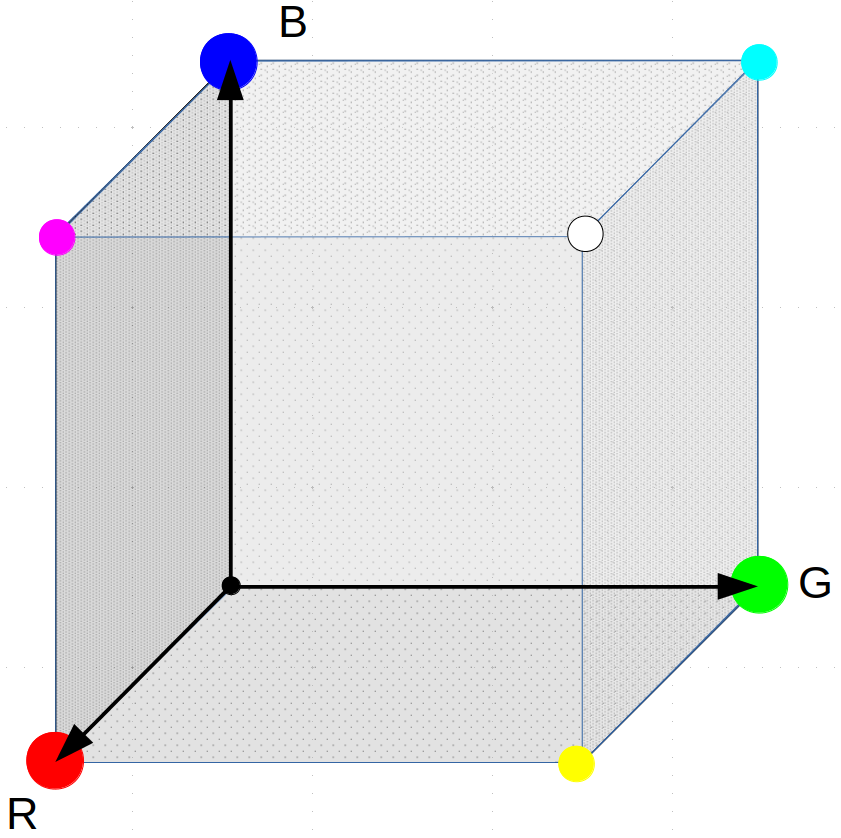
\includegraphics[scale=0.2]{Figures/CuboRGB.png}
    \caption{Espacio RGB}
    \label{fig:RGB_Space}
\end{figure}

\subsubsection{Espacio HSV}
Szeliski describe el espacio HSV, formado con los componentes Matiz (Hue, \textit{H}), Saturación, (Saturation, \textit{S}), Brillantez o Intensidad (Value \textit{V}, Brigtness \textit{B} o Intensity, \textit{I}), mencionando que es una transformación no lineal del espacio de color RGB, correspondiente de igual manera a una tercia de valores que describen el color de interés.

Sonka y Hlavac \cite{czerwinski_definitions_2013} detallan que este espacio de color separa la intensidad y el color, mientras que el matiz y la saturación corresponden a la percepción humana, haciendo muy útil esta representación para desarrollo de algoritmos de procesamiento de imagen, aclarando también que el uso de los valores en RGB puede hacer la manipulación de la imagen propensa a deformaciones de la percepción humana del color. 

Mencionan también que el espacio RGB es utilizado para almacenamiento, procesamiento, codificación o presentación de las imágenes en televisiones, a diferencia del espacio HSV, cuyas aplicaciones se encuentran más enfocadas a la percepción del color y al uso de la imagen en gráficos de computadora.

Los valores asociados a cada uno de los parámetros del espacio HSV son, como se mencionó anteriormente, transformaciones no lineales de los valores  $R,G,B$ y se pueden obtener mediante las ecuaciones de transformación siguientes\cite{burger_digital_2022}:

Siendo:

\begin{equation*}
C_{min} = min(R,G,B), \quad
C_{max} = max(R,G,B), \quad
\Delta = C_{max} - C_{min},
\end{equation*}

Entonces,

\begin{equation*}
    S = \begin{cases*}
  \frac{\Delta}{C_{max}}, & para $C_{max} > 0$.\\
  0, & otros casos,
    \end{cases*}
\end{equation*}

Con el objetivo de mantener los valores de estas transformaciones entre $[0,1]$, se divide entre el valor máximo que será posible que tenga la representación, comúnmente 255.

\begin{equation}
V = \frac{C_{max}}{255},
\end{equation}

\begin{equation*}
R^{'} = \frac{C_{max}-R}{\Delta},  \quad G^{'} = \frac{C_{max}-G}{\Delta},  \quad B^{'} = \frac{C_{max}-B}{\Delta},
\end{equation*}

Posteriormente, dependiendo de cuál de los colores en la representación RGB tuviera el valor máximo, se calcula un valor preliminar del matiz, de la siguiente forma:

\begin{equation*}
    H^{'} = \begin{cases*}
  B^{'} - G^{'}, & cuando $R = C_{max}$,\\
  R^{'} - B^{'}+2, & cuando $G = C_{max}$,\\
  G^{'} - R^{'}+4, & cuando $B = C_{max}$,
    \end{cases*}
\end{equation*}

Lo que resulta en una representación dentro del intervalo $[-1,5]$ y finalmente se obtiene la normalización dentro del intervalo $[0,1]$ como se muestra a continuación.

\begin{equation*}
    H = \frac{1}{6}\cdot\begin{cases*}
  (H^{'}+6), & cuando $H^{'}=0$,\\
  H^{'}, & otros casos,
    \end{cases*}
\end{equation*}

Finalmente, para obtener la representación de la componente H como el correspondiente a un ángulo se multiplica por 360.

\begin{equation*}
    H^{\circ} = H\cdot360
\end{equation*}

Este espacio puede ser gráficamente representado como un prisma circular invertido, donde el radio de la base representa el valor de la saturación (S), La altura del cono representa la intensidad (V), y el matiz (H) se obtiene mediante un ángulo trazado sobre la base del cilindro, comenzando con el color rojo, que se encuentra en 0 grados, el color verde en 120 grados y finalmente el color azul en 240 grados. 

\begin{figure}[H]
\centering
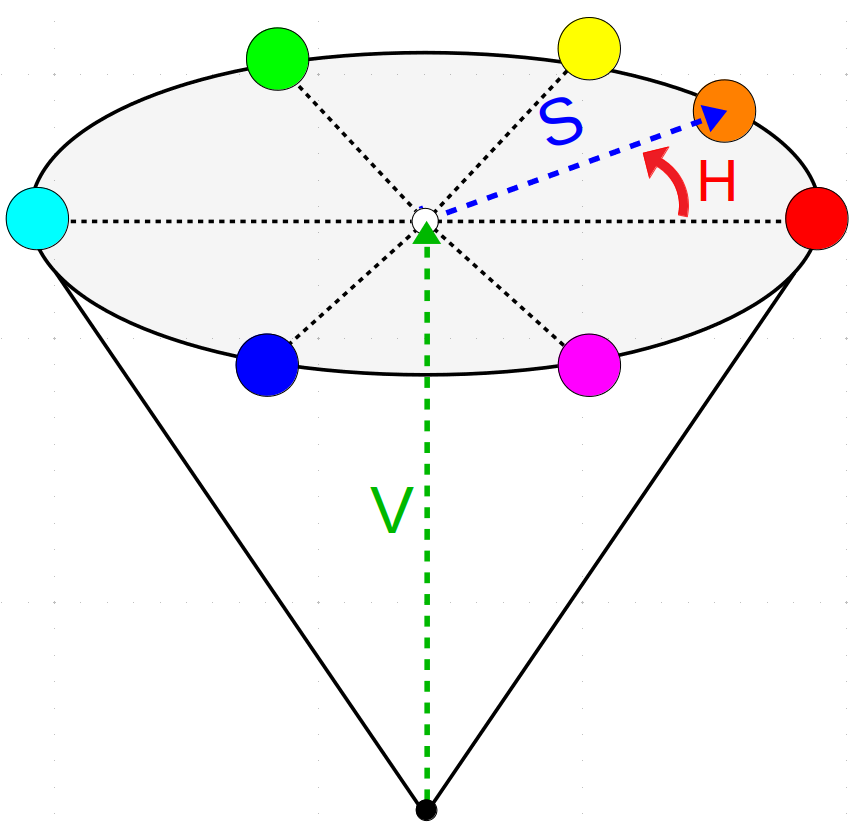
\includegraphics[scale=0.2]{Figures/ConoHSV.png}
    \caption{Espacio HSV, representación cónica}
    \label{fig:HSV_Space}
\end{figure}


\subsection{Segmentación de Imágenes}

En \cite{gonzalez_digital_2002}, los autores comentan que una segmentación robusta es un gran avance en el proceso de procesamiento de una imagen en la cual sea necesario identificar objetos. Adicionalmente, 
Sonka et al. (2018)\cite{sonka_image_2008}, ahondan en las características de la \textbf{segmentación completa} y la \textbf{segmentación parcial}. Explican que en la primera, se obtiene como resultado un conjunto de regiones no superpuestas que corresponden totalmente con \textit{objetos del mundo real} en la imagen de entrada. Mientras que en la segmentación parcial las regiones no corresponden directamente con \textit{objetos del mundo real} presentes en la imagen, sino que aíslan características específicas de la imagen, como la brillantez, el color, la textura, etc. Dada la complejidad asociada a la segmentación completa de las imágenes, para obtenerlas es necesario aplicar niveles más altos de procesamiento a comparación de la segmentación parcial.



Se dice que la segmentación completa de una imagen R es el conjunto finito de regiones $R_{1}, ..., R_{S}$, expresado matemáticamente como: 

\begin{equation*}
R = \bigcup^{S}_{i = 1}, \quad
R_{i} \cap R_{j} = 0, \quad
i \neq j
\end{equation*}

\subsubsection{Umbralización}
La umbralización es una de las herramientas más antiguas para realizar segmentación de imágenes, y tiene como ventaja que no requiere muchos recursos computacionales para realizarla, por lo que es todavía ampliamente utilizada en diferentes aplicaciones. Esta técnica consiste en establecer valores dentro de los cuales se considera aceptable la característica de interés.

Este proceso corresponde a la transformación de una imagen de entrada $f$ a una salida segmentada, una imagen binaria $g$, de la siguiente forma:

\begin{equation*}
g(i,j) =\begin{cases*}
1, & para $f(i,j) \geq T$,\\
0, & para $f(i,j) < T$ \end{cases*} 
\end{equation*}
\phantom{saltodelinea}\\

Donde $T$ representa el umbral (Threshold). Después de esta trasnformación, todos los pixeles dentro de la imagen que se encuentren dentro del/los umbrales definidos tendrán un valor de 1 y a aquellos que no satisfagan la condición se les asigna el valor 0 (o vice versa) \cite{sonka_image_2008}. \phantom{saltodelinea}



González y Woods \cite{gonzalez_digital_2002} describen el proceso de segmentación de imágenes en el espacio HSV de la siguiente manera:
\begin{itemize}
    \item Separar la imagen en sus componentes HSV.
    \item Reconocer las zonas de la imagen (y los valores de los píxeles) donde se encuentran las características de interés.
    \item Establecer los umbrales de los valores HSV que determinan los píxeles que representan la información de valor.
    \item Umbralizar: generar una máscara binaria con las regiones donde se encuentran dichos valores.
    \item Utilizar la máscara y la imagen original para aislar las regiones de interés de la imagen.
\end{itemize}


\subsection{Operaciones Morfológicas}

González y Wood explican también que bajo el contexto de procesamiento de imágenes la \textit{morfología matemática} hace alusión a una herramienta para extraer los componentes de la imagen que son útiles para la representación y descripción de la forma de una región. Indica además que el lenguaje que se ha de utilizar para este procesamiento es la teoría de conjuntos y resaltan que los conjuntos en \textit{morfología matemática} representan objetos en una imagen.
Debido a la relación mencionada entre el procesamiento morfológico de la imagen y la teoría de conjuntos, se explican en enseguida algunos conceptos iniciales.

\subsubsection{Teoría de Conjuntos}
Sea $A$ un conjunto perteneciente a $Z^2$. Si $a = (a_{1}, a_{2})$ es un elemento de $A$, se representa de la siguiente forma: $a \in A$. De forma similar, si $a$ no es un elemento de $A$, se representa como: $a\notin A$.

Aquel conjunto en el cual no hay elementos se conoce comúnmente como el conjunto \textit{nulo} o conjunto \textit{vacío} y se utiliza el símbolo $\oslash$.

Un \textbf{conjunto} se representa por lo contenido entre dos llaves: $\{\cdot\}$ y los elementos de los conjuntos que son de nuestro interés en este contexto son los píxeles que componen una imagen digital.

Si todos los elementos de A se encuentran también en el conjunto B, se dice que el conjunto A es un \textbf{subconjunto} del B y se escribe de la siguiente forma:

\begin{equation*}
A\subseteq B
\end{equation*}

La \textbf{unión} $C$ de los conjuntos $A$ y $B$ es aquel conjunto al que pertenecen todos los elementos ya sea de A, B o de ambos y se expresa como:

\begin{equation*}
C = A \cup B
\end{equation*}

La \textbf{intersección} $D$ de dos conjuntos es el conjunto que contiene a los elementos que pertenecen a $A$ y a $B$:

\begin{equation*}
D = A \cap B
\end{equation*}

\begin{figure}[H]
\centering
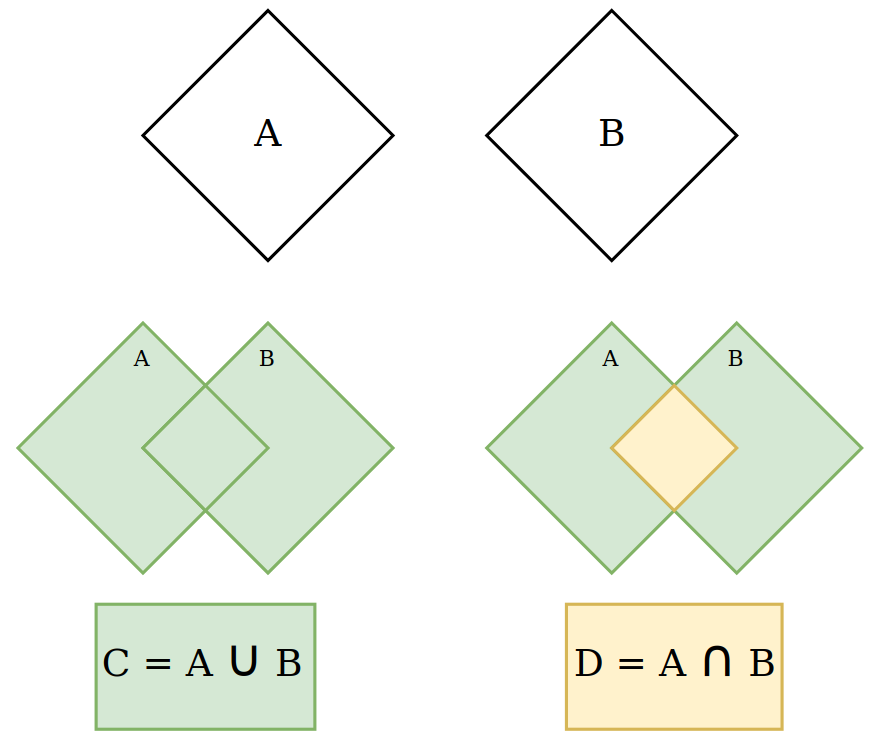
\includegraphics[scale=0.3]{Figures/Conjuntos.png}
    \caption{Unión e Intersección de Conjuntos}
    \label{fig:UnioneInterseccion}
\end{figure}

Se dice que dos conjuntos son \textbf{mutuamente excluyentes} si no tienen ningún elemento en común, 

\begin{equation*}
A \cap B = \oslash
\end{equation*}

El \textbf{complemento} del conjunto A es el conjunto de todos aquellos elementos que no pertenecen a A.

\begin{equation*}
A^{C} = \{\omega \mid \omega \notin A\}
\end{equation*}
Dado el conjunto Universal $U$:
\begin{figure}[H]
\centering
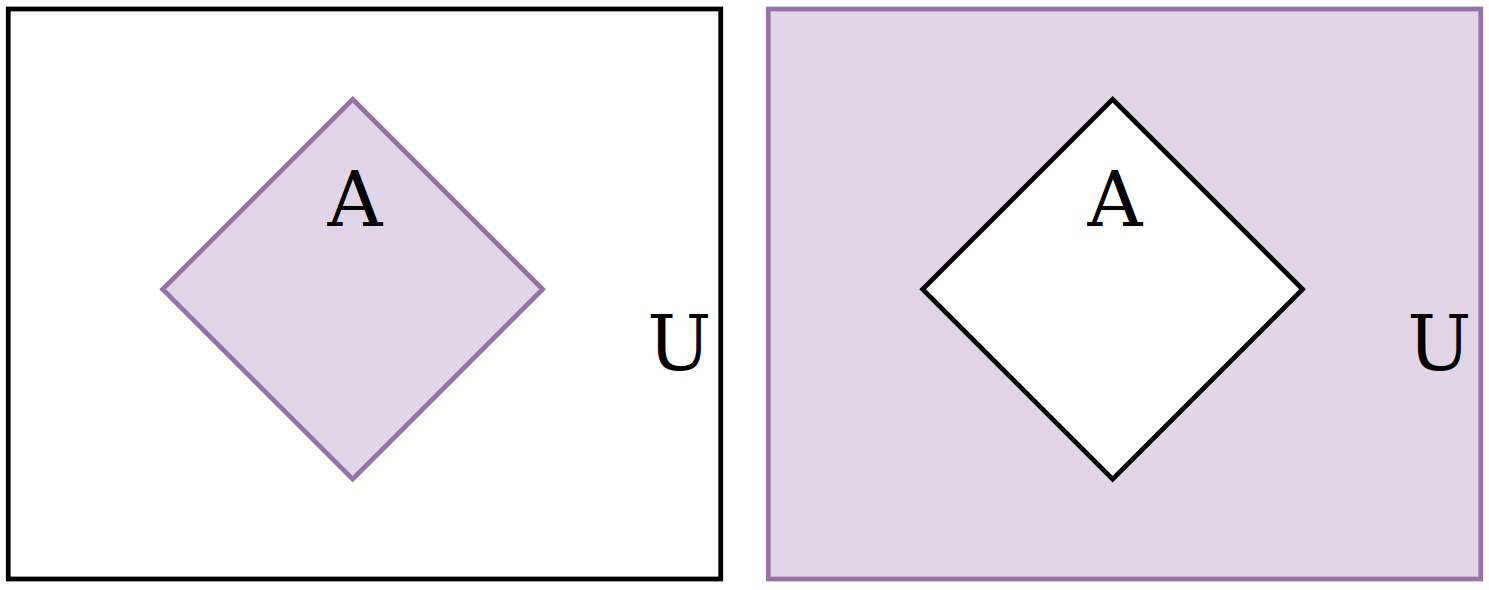
\includegraphics[scale=0.17]{Figures/Conjuntos_Complemento.png}
    \caption{Complemento}
    \label{fig:Complemento}
\end{figure}

La \textbf{diferencia} entre dos conjuntos $A$ y $B$ representada como $A-B$, es el conjunto de elementos que pertenecen a A pero no a B se define como:

\begin{equation*}
A - B = \{ \omega \mid \omega \in A, \omega \notin B \} = A \cap B^{C}
\end{equation*}

\begin{figure}[H]
\centering
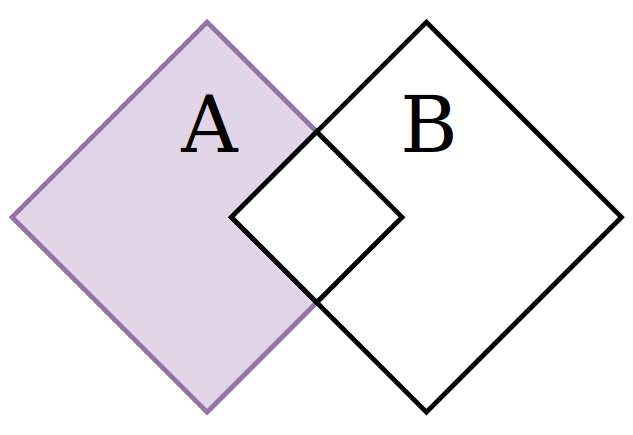
\includegraphics[scale=0.17]{Figures/Conjuntos_Resta.png}
    \caption{Diferencia}
    \label{fig:Diferencia}
\end{figure}

La reflexión del conjunto B se define como:

\begin{equation*}
\hat{B} = \{ \omega \mid \omega -b, \textup{ para } b \in B \}
\end{equation*}

\begin{figure}[H]
\centering
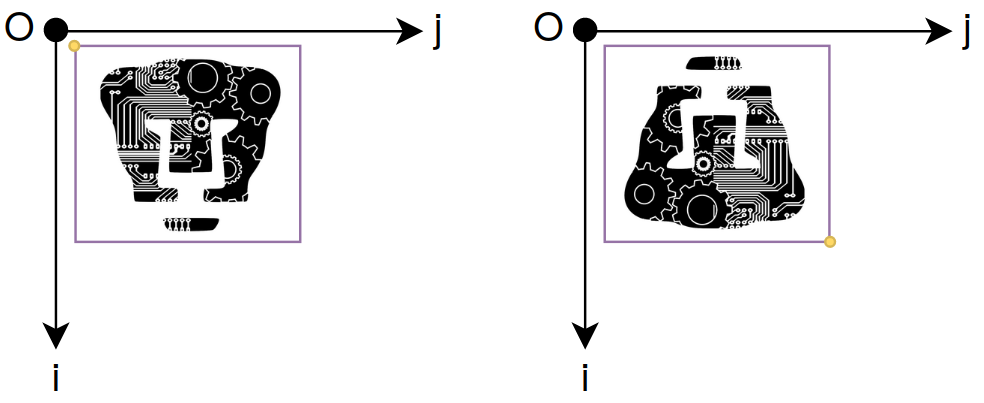
\includegraphics[scale=0.32]{Figures/Reflexion.png}
    \caption{Reflexión}
    \label{fig:Reflexion}
\end{figure}

La traslación del conjunto A al punto $Z = (z_{1}, z_{2})$, representada como $(A)_{z}$, se define como:

\begin{equation*}
(A)_{z} = \{ c \mid c = a+z, \textup{ para } a \in A \}
\end{equation*}

\begin{figure}[H]
\centering
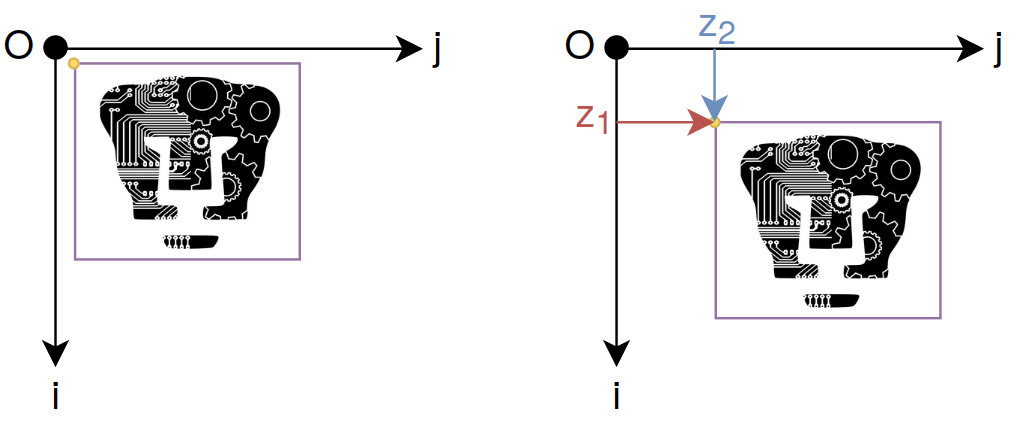
\includegraphics[scale=0.32]{Figures/Traslacion.png}
    \caption{Traslación}
    \label{fig:Traslacion}
\end{figure}

En las figuras \ref{fig:Reflexion} y \ref{fig:Traslacion} el origen de las imágenes originales se encuentra resaltado con un punto amarillo.

\subsubsection{Operaciones Lógicas}

Comúnmente el procesamiento morfológico se realiza sobre imágenes en blanco y negro, es decir, imágenes en donde los únicos valores posible para los píxeles son 1 y 0, esto permite que se utilicen operaciones binarias sobre los píxeles de la imagen. 
Algunas de las operaciones binarias que con más frecuencia se utilizan para el procesamiento de imágenes son las operaciones \textbf{AND}, \textbf{OR}, y \textbf{NOT}. Las dos primeras permiten operar entre dos o más imágenes, como en el caso de aplicar una máscara sobre una imagen, utilizando la operación AND. En la Figura \ref{fig:LogicOp} se muestra el comportamiento de estas operaciones lógicas.

\begin{figure}[H]
\centering
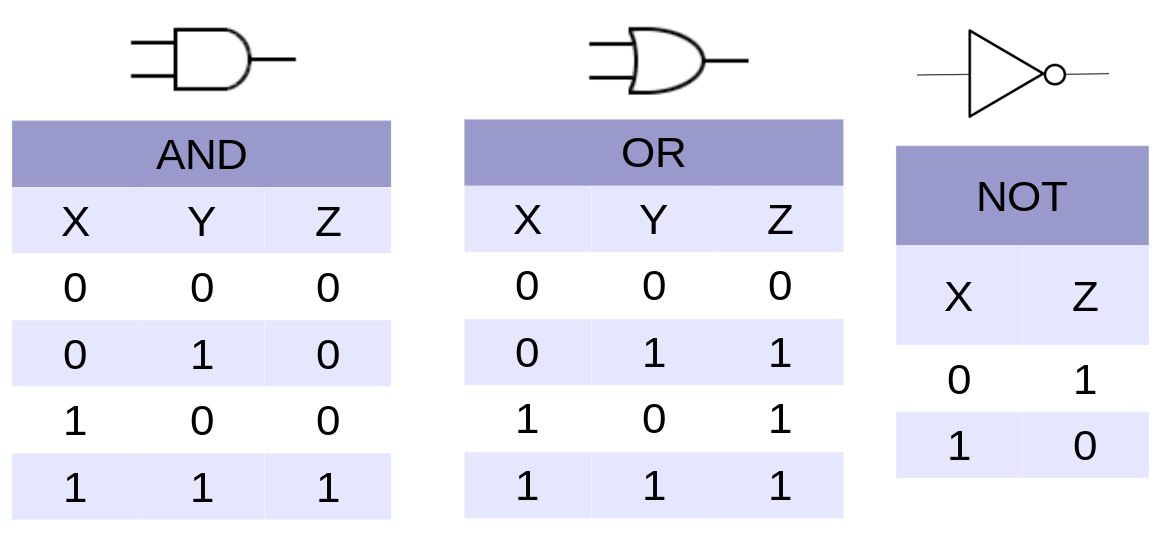
\includegraphics[scale=0.2]{Figures/CompuertasLogicas.png}
    \caption{Operaciones Lógicas AND, OR y NOT}
    \label{fig:LogicOp}
\end{figure}

Estas operaciones tienen comportamientos similares a los mencionados en teoría de conjuntos, con la limitante de que las operaciones lógicas solo pueden ser utilizadas con valores binarios después de la umbralización de los valores de los píxeles de la imagen, en la Figura \ref{fig:LogicOpIMG} se observa un ejemplo del comportamiento de estas operaciones en una imagen binaria.
\begin{figure}[H]
\centering
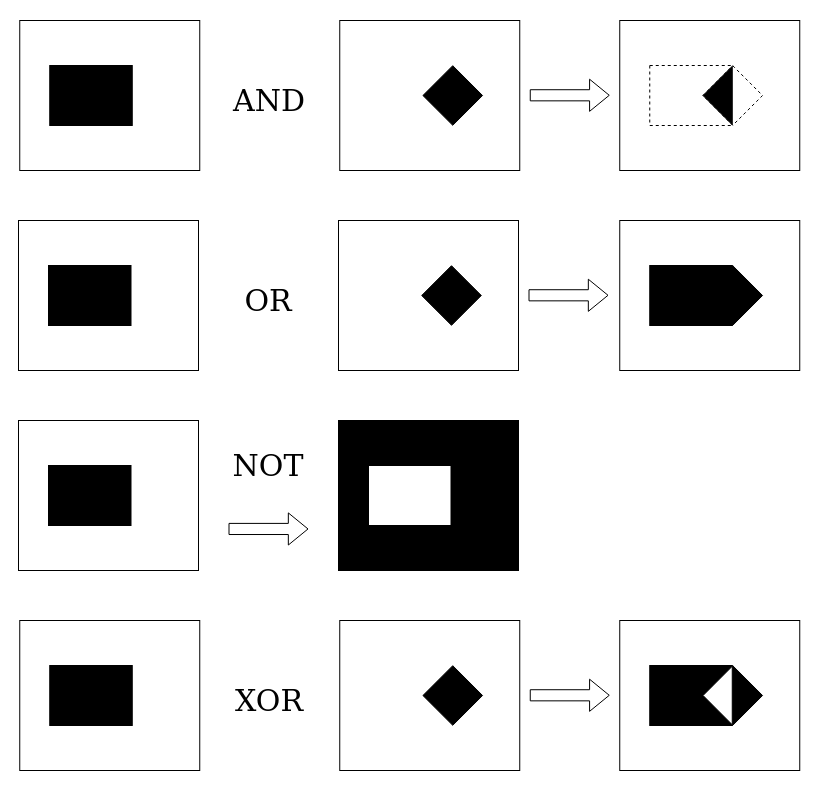
\includegraphics[scale=0.3]{Figures/LogicOp_IMG.png}
    \caption{Operaciones Lógicas Aplicadas a Imagen}
    \label{fig:LogicOpIMG}
\end{figure}

\subsubsection{Dilatación y Erosión}

Estas operaciones se consideran básicas dentro el procesamiento morfológico de las imágenes y algunas  de las técnicas más avanzadas que se utilizan, se basan en ellas.

\emph{Dilatación}\\
Siendo $A$ y $B$ dos conjuntos en $Z^2$, la dilatación de $A$ y $B$, expresada como $A \oplus B$, se define como:

\begin{equation*}
A \oplus B = \{ z \mid (\hat{B})_{Z} \cap A \neq \oslash \}
\end{equation*}

Para obtener esta ecuación es necesario obtener la reflexión de $B$ sobre su origen e invirtiendo su reflexión en $z$. La dilatación de A por B es el conjunto de todos los desplazamientos de $z$, tal que B y A se sobreponen por al menos un elemento. De acuerdo con esta descripción, es posible re-escribir la anterior definición como:

\begin{equation*}
A \oplus B = \{ z \mid [(\hat{B})_{Z} \cap A] \subseteq A \}
\end{equation*}

en estas ecuaciones, el conjunto $B$ es comúnmente mencionado como el \textit{elemento estructurante} de la dilatación y otras operaciones.

Vale la pena mencionar que esta definición de la operación dilatación coincide con el proceso para realizar la convolución, dado que de forma similar se \textit{invierte} uno de los operandos y se recorre sobre el otro elemento de la operación. Es importante recalcar que la convolución es una más de las operaciones que con frecuencia se utilizan para el procesamiento de imágenes, por ejemplo para el filtrado de las imágenes, al hacer la convolución de la forma matricial de la imagen con la matriz que represente el filtro que se busca aplicar. 

\emph{Erosión}


Para los conjuntos $A$ y $B$, pertenecientes a $Z^{2}$, la operación erosión, representada como $A \ominus B$, se define como:

\begin{equation*}
A \ominus B = \{ z \mid (B)_{Z} \subseteq A \}
\end{equation*}

Es decir, la erosión aplicada a estos conjuntos resulta en el conjunto de todos los puntos $z$, tal que B (traducido en puntos $z$), que son contenidos en A.

En la figura \ref{fig:Ero+Dil} se muestra un ejemplo de los efectos de la operación morfológica, a)Imagen original, b)Matriz de 3x3 como Elemento estructurante, c)Operación Erosión aplicada a la Imagen Original, d)Operación Dilatación aplicada a c).

\begin{figure}[H]
\centering
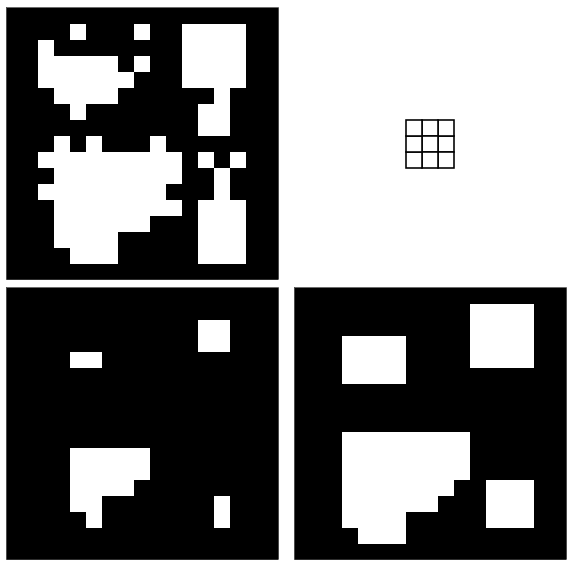
\includegraphics[scale=0.53]{Figures/ErosDil_NoGrid.png}
    \caption{Operaciones Morfológicas: Dilatación y Erosión}
    \label{fig:Ero+Dil}
\end{figure}

Como es posible notar en el ejemplo, estas dos operaciones no son estrictamente inversas entre sí. Además, dado que al realizar la operación erosión se pierde información sobre los detalles de la imagen original, es imposible recuperarla aplicando la dilatación. Adicionalmente, elemento estructurante tiene gran influencia en el resultado que se obtendrá, dado que una modificación en sus dimensiones o su forma resulta en una evidente modificación de la imagen final, un ejemplo de esto puede verse en la figura \ref{fig:Dil_ES2}, utilizando nuevamente  \ref{fig:Ero+Dil}, inciso c) como imagen base.

\begin{figure}[H]
\centering
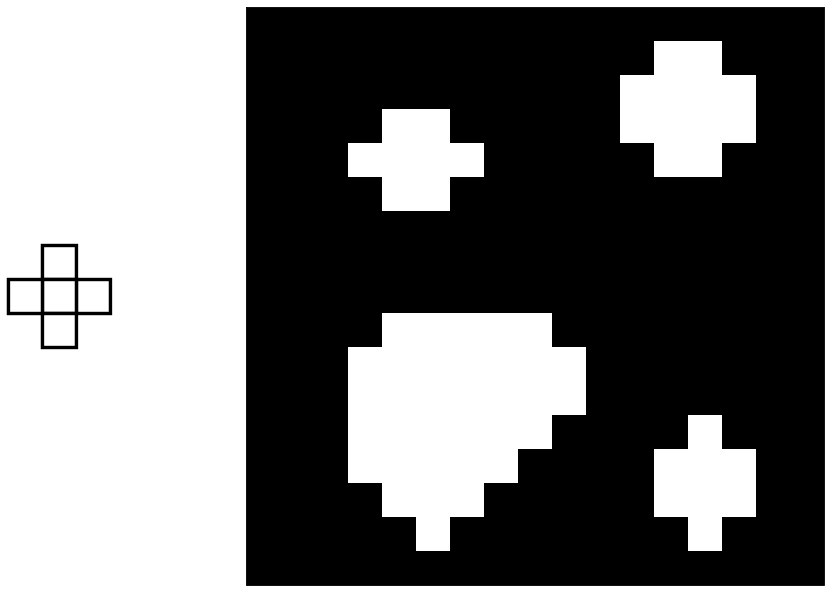
\includegraphics[scale=0.25]{Figures/Dil_ES2.png}
    \caption{Dilatación aplicada con distinto Elemento Estructurante}
    \label{fig:Dil_ES2}
\end{figure}

%%Detección de Bordes y Filtro Gaussiano

\section{Reconocimiento de Objetos}
Una de las partes fundamentales de la visión computacional es la habilidad de reconocer objetos dentro de las imágenes que son procesadas, para lo cual se utilizan algoritmos de reconocimiento de patrones que nos permiten clasificar objetos o regiones dentro de la imagen, haciendo posible entender mejor los elementos que la componen.

Como se ha mencionado anteriormente, para nosotros las tareas asociadas a la visión son actividades que llevamos a cabo de manera natural, sin que requiera un esfuerzo consciente en la mayoría de los casos y, teniendo ya sea un ejemplo visual o bien una descripción sobre las características de nuestro objeto de interés, somos capaces de identificarlo dentro del entorno. Con el objetivo de reconocer los objetos mediante el análisis computacional de las imágenes, es imprescindible conocer las características de dichos objetos, así como de las clases a las que pertenecen.

De acuerdo con Sonka \cite{sonka_image_2008}, el diseño de una adecuada representación del conocimiento es la parte más importante de la resolución del problema del entendimiento y se refieren a las descripciones y las características como una representación de \textit{bajo nivel}, aclarando que no pueden ser consideradas en sí mismas como representaciones del conocimiento, aunque sí pueden ser usadas como parte de una estructura de representación más compleja.

Se ha dicho antes que como humanos podemos utilizar descripciones verbales o escritas de la apariencia de un objeto y utilizar esa información para identificarlos, sin embargo, para que una máquina pueda replicar este comportamiento es necesario tener  una representación de esta descripción que sea posible procesar matemáticamente. En este contexto las representaciones se hacen de forma numérica, asociando cada característica a una magnitud escalar. 
Para poder hacer la clasificación de objetos complejos es preferible que la descripción incluya la representación de varias propiedades del objeto en cuestión. Al conjunto de características representadas numéricamente se le conoce como \textbf{vectores de características}, que se utilizan como entradas para los algoritmos de reconocimiento. A este vector de características se le conoce también como \textbf{patrón}.

En el reconocimiento se les asignan clases a los objetos. En este proceso, el número de clases existentes es frecuentemente conocido desde el planteamiento del problema. Dependiendo del conjunto de las características de la clase que las propiedades del objeto satisfacen, se asignan a una u otra; el elemento encargado de esta la tarea de clasificación es conocido como \textbf{clasificador}.

El proceso principal para el reconocimiento de patrones se muestra en la figura \ref{fig:Pat_Recog}, donde podemos ver que un objeto es la entrada de un bloque de procesamiento del cual se obtiene el \textbf{patrón} del objeto, es decir, se construye el \textbf{vector de características} al aislar y cuantificar las propiedades del objeto. Este vector es posteriormente ingresado al clasificador y como salida del proceso se obtiene la clase a la que el objeto pertenece.

\begin{figure}[H]
\centering
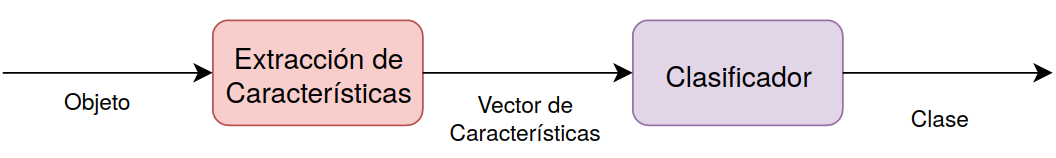
\includegraphics[scale=0.3]{Figures/Clasificacion.png}
    \caption{Reconocimiento de Objetos}
    \label{fig:Pat_Recog}
\end{figure}

Dependiendo de la aplicación para la cual se busque realizar el reconocimiento serán importantes diferentes características de los objetos. Además, las características de los recursos disponibles también encontrarán cambios. Debido a esto, se han desarrollado muchas y muy variadas técnicas de reconocimiento, utilizando cada vez diferentes características y técnicas de procesamiento de la información.
Treiber \cite{treiber_introduction_2010} en 2010, menciona que bajo los siguientes parámetros es posible definir una clasificación de los métodos de reconocimiento de objetos:

\begin{itemize}
    \item Representación de objetos: basados en la geometría (silueta, forma) o la apariencia (regiones de imagen que pertenecen al objeto).
    \item Alcance de la información sobre los objetos: características locales (descripción de una parte del objeto) o globales (información sobre el área, perímetro, etc).
    \item Variación esperada de los objetos: qué tan diferentes pueden ser los objetos dentro de una misma clase.
    \item Calidad de los datos de la imagen: dependiendo de la aplicación es posible que las imágenes a procesar contengan ruido, oclusiones o menor definición, por lo que requieren más procesamiento.
    \item Estrategia de comparación: en el proceso de reconocimiento es necesario un paso en el cual se realiza una comparación entre la similitud entre la imagen analizada y la referencia. Dependiendo del algoritmo de comparación usado cambian también los parámetros requeridos.
    \item Alcance de la información de los elementos utilizados en la comparación: el autor propone una división en las siguientes tres categorías: valores sin procesar de los píxeles de intensidad, características de bajo nivel (bordes) y alto nivel (líneas o arcos). 
\end{itemize}

Una vez establecidas estas condiciones, el autor lista algunos métodos de reconocimiento de objetos:

\begin{itemize}
    \item \textbf{Métodos globales}\\ Buscan modelar y encontrar los objetos únicamente con características globales.
    \item \textbf{Métodos basados en Transformación y Búsqueda}\\ La pose del objeto se determina buscando el espacio de transformaciones entre el modelo y la información de la imagen
    \item \textbf{Métodos basados en Correspondencia Geométrica}\\ Utilizan las relaciones geométricas entre varias parte del objeto y establece correspondencias entre el modelo y las características de la imagen.
    \item \textbf{Métodos basados en descriptores}\\ Buscan identificar los objetos utilizando descriptores, normalmente de la apariencia de los objetos en regiones locales cerca de los puntos de interés. 
\end{itemize}

El proceso utilizado en este proyecto corresponde a la última categoría de las anteriores,y fue elegido dado que su implementación no requiere muchos recursos computacionales y es suficientemente rápido para la aplicación propuesta. Además, claro, que las características de los objetos de interés lo permiten.


\section{Máquinas de Estado}

Cuando se habla de máquinas de estados nos referimos a un modelo computacional con el cual se representan procesos de lógica secuencial. En este modelo cuenta con conjuntos de entradas, salidas y el funcionamiento del sistema se compone por estados y funciones de transformación. En este modelo se establece que en cualquier momento de la ejecución es posible estar en uno y solo un estado a la vez, y el salto entre estados se condiciona por medio de las ya mencionadas funciones de transformación, que determinan si se realiza el cambio a otro de los estados.

Czerwinski y Kania \cite{czerwinski_definitions_2013}, enuncian la definición matemática de la Máquina de Estados Finitos (FSM) utilizando un vector de 5 elementos, $\{X,Y,S,\delta,\lambda\}$, donde $X$ corresponde a un espacio de entradas finitas, $Y$ al espacio de salidas finitas, $S$ a un conjunto de estados finitos, $\delta$ representa la función de transformación y $\lambda$ la función de salidas. En este caso, la función de transición de una Máquina de estados finitos determina el siguiente estado ($S^+$), y se refiere al mapeo $\delta: X \times S \to S $.


Dentro de las máquinas de estados finitas se encuentran dos grandes clasificaciones, las máquinas Moore y las máquinas Mealy, que reciben su nombre de los investigadores Eduard F. Moore y George H. Mealy, que desarrollaron \textit{la teoría del autómata}. En el planteamiento de la máquina de Moore las salidas dependen únicamente del estado actual de la máquina, expresando este comportamiento en términos de los vectores definidos anteriormente se obtiene: $\lambda: S \to Y$. Por el contrario, en las máquinas Mealy las salidas dependen tanto del estado actual como de las entradas actuales del sistema. Así, la función de salida se puede representar como: $\lambda: X \times S \to Y$.


\section{Sistemas expertos}
 
A mediados del Siglo XX, cuando el concepto de Inteligencia Artificial comenzaba a popularizarse, su aplicación principal se centraba en planeación y solución de problemas. En aquel momento era difícil imaginar que décadas más tarde las aplicaciones más importantes se encontraran en ingeniería del conocimiento y en sistemas expertos. En 1982 el profesor Edward Feigenbaum de la Universidad de Stanford, uno de los pioneros en el desarrollo de tecnología de sistemas expertos, definió un sistema experto como "un programa computacional que utiliza procedimientos de inferencia para resolver problemas que son suficientemente complicados para requerir conocimiento humano especializado para su solución."
\cite{giarratano_zhuan_2002}

En 2020, 38 años más tarde de esta definición, Gupta \cite{gupta_artificial_2020} refiere que un sistema experto es un programa computacional que emula la capacidad de razonar y el comportamiento de un humano con el conocimiento y experiencia de un experto en un campo específico. También indica que los sistemas expertos son utilizados para resolver problemas complejos utilizando el conocimiento almacenado en una base de datos en forma de reglas. 

De acuerdo con Liebowitz \cite{liebowitz_handbook_2019} la adquisición de conocimiento es el proceso de extraer, estructurar y organizar el conocimiento de diferentes fuentes, usualmente humanos expertos en un área, de forma tal que la habilidad de solucionar problemas pueda ser capturada y transformada para que una computadora sea capaz de leerla. De acuerdo con este autor: "Sin conocimiento explícitamente representado, un sistema experto no es más que un programa de computadora."

Gupta y Liebowitz señalan también que uno de los pasos intermedios entre la adquisición de conocimiento y la implementación de sistemas expertos es la intervención de un Ingeniero de conocimiento, un individuo que estudia la forma en que los expertos toman decisiones y lo traduce a reglas en términos comprensibles para la máquina. A partir de esto, Gupta menciona que los sistemas expertos son también conocidos como sistemas basados en conocimiento o sistemas expertos basados en conocimientos, así como sistemas basados en reglas, y que se consideran como Inteligencia Artificial Aplicada. 

\section{Manipulación del Robot}
Siendo la manipulación de objetos un de los objetivos principales de este proyecto es pertinente explicar la forma en que le es posible al robot tomar los objetos que se espera que transporte. Para esto, es necesario realizar el análisis cinemático del robot, que consiste en el estudio de la relación que guarda el efector final respecto a la estructura que compone el manipulador del robot, es decir el comportamiento que debe tener cada articulación del robot para que el efector final pueda posicionarse en las coordenadas finales deseadas para el comportamiento esperado del robot.

Para realizar este análisis es necesario conocer el número de grados de libertad con los que cuenta el manipulador que se usará, así como el tipo de articulaciones con las que cuenta, los ejes en los que actúa cada una y sus limitaciones de movimiento.

Ceccareli \cite{ceccarelli_fundamentals_2022}, explica que es posible formular numéricamente esta situación para determinar las coordenadas de las articulaciones $q_{i}(i=1,...,N)$ como funciones de la configuración del manipulador. Amplía diciendo que la formulación debe considerar aspectos numéricos que están relacionados a la existencia de soluciones  y a la multiplicidad de soluciones.

Los autores describen que la existencia de soluciones hace referencia a que cuando una configuración dada no se encuentre dentro del rango de movilidad del manipulador, la solución numérica de la cinemática inversa no puede ser obtenida dentro del espacio de trabajo del manipulador. Para lo cual se requiere conocer el rango de movilidad de las articulaciones y los límites del espacio de trabajo antes de unir la solución numérica. En términos matemáticos, el cumplimiento de los límites del espacio de trabajo significa que las soluciones que se obtengan pertenezcan al dominio de los números reales.

De forma similar, es posible encontrar múltiples soluciones  debido a la naturaleza \textit{altamente no lineal} de la posición cinemática de los manipuladores, es decir las diferentes configuraciones en las que se pueden posicionar los actuadores para que el efector final llegue a una coordenada determinada dentro del espacio de trabajo. 

\section{Estado del Arte}

Durante el desarrollo de este proyecto fue notable que dentro del entorno en que se plantea su desarrollo, los equipos que previamente han participado proceden sin utilizar procesamiento de imágenes en gran medida, usando en su mayoría sensores de proximidad y similares. Si bien las piezas que se tiene como objetivo que el robot identifique y sujete cuentan con características similares en forma, el color es una de las diferencias más evidentes tanto entre ellas como en relación al ambiente en que se encuentran de forma regular y se considera una característica de mucha utilidad en detección de objetos. Aunque es cierto que el entorno de la competencia en que se plantea la evaluación del comportamiento de este desarrollo se encuentra bajo condiciones controladas y es evidentemente una simulación de las condiciones de ejecución reales de un ambiente industrial, se sigue considerando conveniente el uso de cámaras y procesamiento de imágenes que permitan explotar la mayor cantidad de recursos disponibles, además de que este enfoque ofrece un aumento en la vesatilidad de la información recabada sobre el desempeño de lo sistemas.

\subsection{Antecedentes en RoboCup Logistics}
Dentro de la documentación disponible en el sitio web oficial de la RoboCup se listan los \textit{Team Description Paper} (TDP), donde se describen las técnicas utilizadas en la competencia por los equipos participantes. En estos documentos se encuentran pocos referentes de cámaras utilizadas en secciones de la competencia fuera de la localización de los códigos ARUCO en las estaciones. Estas cámaras se encuentran típicamente en la parte inferior de los robots. En el TDP presentado por el equipo austriaco GRIPS (Graz Robust and Intelligent Production System) para su participación en la competencia del 2021 \cite{furbaß_robocup_2021}, el equipo describe que, para la alineación con la banda transportadora, el robot inicia en una posición de referencia cercana a la estación, desde la cual se utiliza el sensor láser y el código ARUCO que se encuentra en sus paredes para realizar la alineación. El equipo reconoce que este primer alineamiento, combinando la información de estas dos fuentes, no es muy preciso. Por lo anterior, utilizan una segunda cámara que se encuentra en una posición más elevada para los movimientos más finos del proceso. 

\begin{figure}[H]
    \centering
    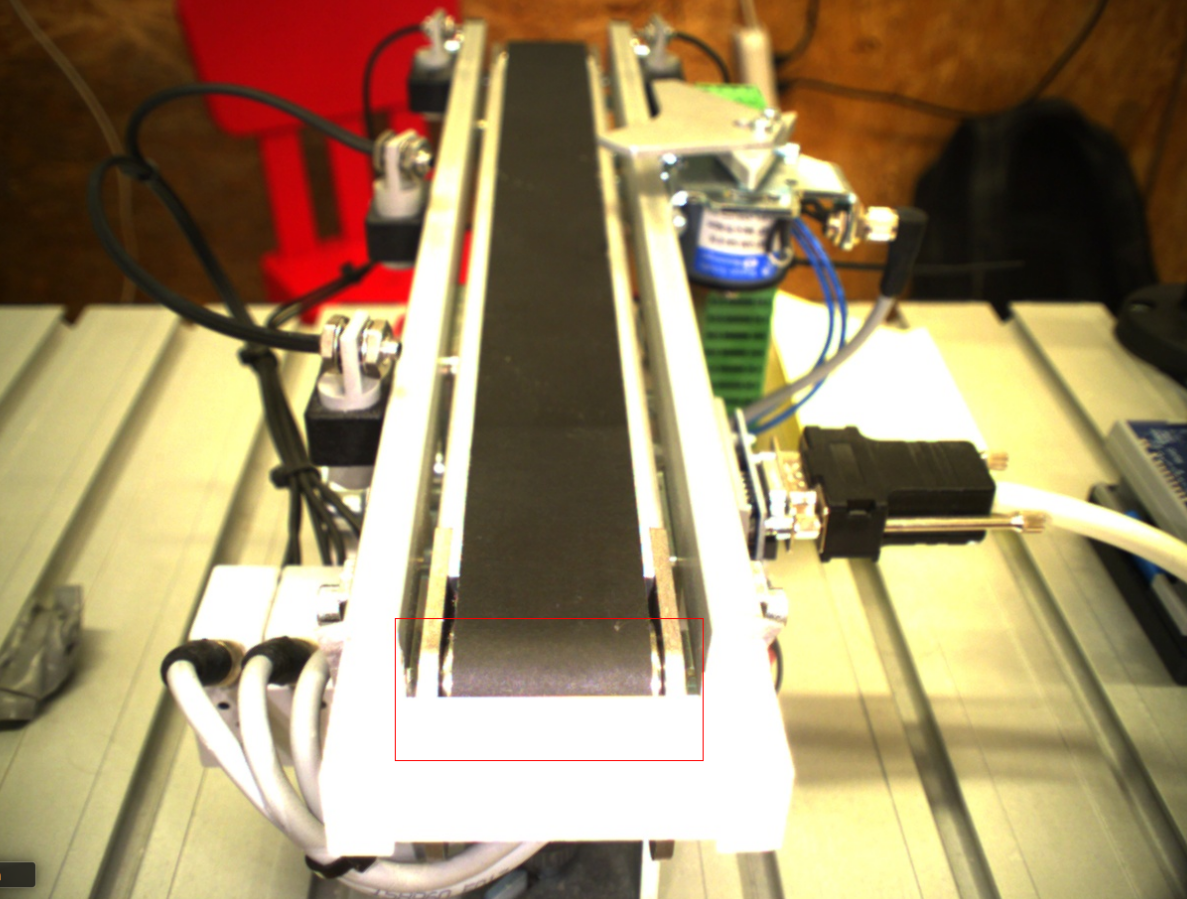
\includegraphics[scale=0.15]{Figures/Conveyor_GRIPS_TDP.png}     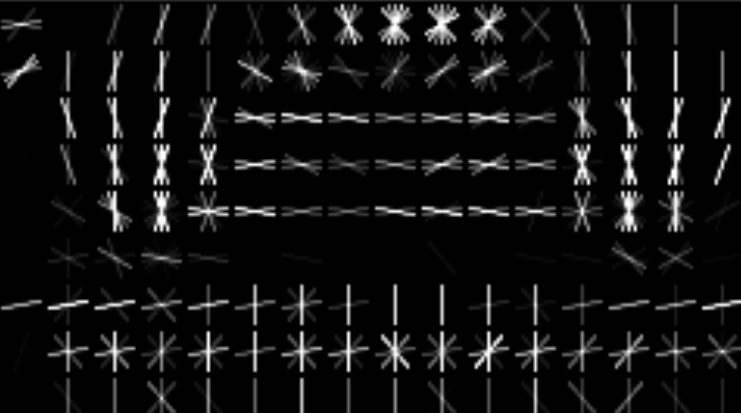
\includegraphics[scale=0.2]{Figures/Conveyor_HOG_GRIPS_TDP.png}
        \caption{Detección de Histogramas de Gradientes Orientados \cite{furbaß_robocup_2021}}
        \label{fig:HOG_GRIPS}
    \end{figure}

Con este objetivo implementaron un detector de Histogramas de Gradientes Orientados (HOG, por sus siglas en inglés). con el cual detectan la posición de los diferentes elementos de interés dentro del espacio de trabajo. Los autores describen que el HOG identifica regiones de la imagen, en las cuales se encuentran las características más representativas de los elementos ambientales. Para este punto del proceso, las características mencionadas ya eran conocidas por el algoritmo, para lo cual fue necesaria la toma de imágenes de entrenamiento y evaluación. Una vez que se aisla la zona de interés, el HOG genera un conjunto de características. Los autores mencionan que las imágenes de entrenamiento se utilizan para encontrar las características que describen las regiones de interés y las imágenes de evaluación para verificar que dichas características realmente coincidan con los objetos, como es típico en procesos de este tipo.

La descripción del proceso provista por los autores especifica que, una vez que el robot se encuentra en la posición adecuada, la cámara superior toma 4 imágenes con diferentes iluminaciones, logrados con fuentes de luz con las que cuenta el robot. Este esfuerzo se realiza con el objetivo de mitigar los errores debidos a las variaciones de iluminación naturales, y promover una correcta detección de las características de interés aún si las condiciones en las que se encuentra la estación no corresponden con las imágenes con las que fue previamente entrenado el algoritmo. Adicionalmente, para intentar robustecer el procedimiento, los autores utilizaron varios HOG en diferentes objetos, entrenando cada uno con diferentes conjuntos de imágenes, buscando diversificar las características de entrenamiento para su algoritmo de reconocimiento. En la figura \ref{fig:Robotino_GRIPS} se observan las modificaciones que el equipo GRIPS llevó a cabo en su robot hasta la edición 2021 de la competencia. Sin embargo, actualmente la implementación ya no cuenta con la cámara elevada y la estructura superior ha sido descartada.

\begin{figure}[H]
    \centering
    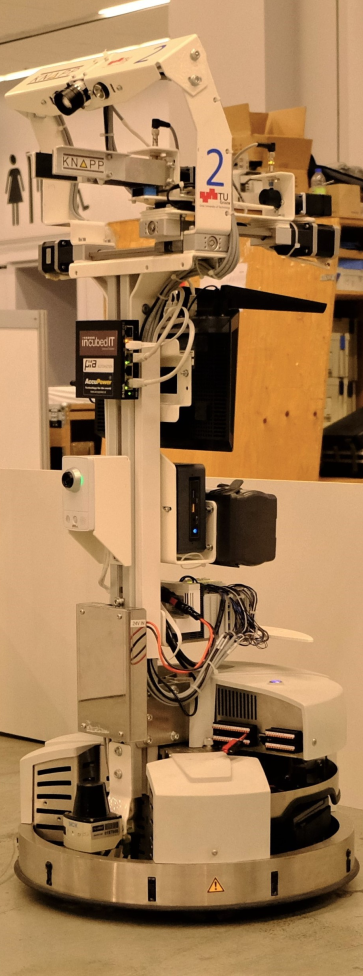
\includegraphics[scale=0.25]{Figures/RobotinoGRIPS_Old.png}
        \caption{Robotino modificado - GRIPS \cite{furbaß_robocup_2021}}
        \label{fig:Robotino_GRIPS}
\end{figure}

Para realizar la tarea de alineación, el equipo utiliza una combinación de sensores de proximidad que se encuentran debajo de y en el centro de la pinza del manipulador, utilizando también un movimiento que combina la alineación del robot con la máquina y del manipulador con la banda transportadora.

De manera similar, dentro del desarrollo del trabajo para la siguiente participación en la competencia, se planea integrar sensores de proximidad, combinando los avances obtenidos del presente proyecto, con las herramientas vistas durante lo experimentado en la edición 2023. Cabe mencionar que la configuración mecánica de los manipuladores de ambos equipos es y seguirá siendo distinta. 

\subsection{Segmentación por Color}
Debido a su bajo costo de procesamiento los algoritmos de segmentación de imágenes por color siguen siendo utilizados constantemente en gran variedad de aplicaciones. Una de ellas, es la detección de enfermedades en plantas dentro de la industria agrícola. En 2022, Hassan et.al. \cite{HASAN20227212} 



\input{Ch03_Detección_de_objetos}
\input{Ch04_Planeación_de_movimientos}
\input{Ch05_Planeación_de_acciones}
\chapter{Resultados}
    \section{Herramientas}
    Para lograr los objetivos planteados para el desarrollo de este proyecto se utilizaron varias herramientas de software y de hardware, las cuales hicieron posible la recopilación de los datos necesarios, así como la ejecución de las acciones planteadas como requisitos del proceso planteado.
    Se ha hecho suficiente hincapié en que el objetivo principal de este proyecto es el aprovechamiento de los datos recabados por una cámara RGBD. En este caso, el dispositivo utilizado para la obtención de la imagen y la nube de puntos es el \textbf{Kinect}, un dispositivo distribuido por la empresa \textbf{Microsoft}, que en 2010 fue lanzado al mercado como accesorio para la consola de videojuegos XBOX 360. Adicionalmente, como base del robot móvil se utilizó la plataforma de desarrollo \textbf{Robotino} perteneciente a la empresa FESTO.

    
        \subsection{Herramientas de software}
            \subsubsection{ROS}
            En 2018 Edgar Vázquez realiza una breve de descripción del sistema ROS, en la cual comenta que el objetivo principal es dar soporte a la reutilización de código en la investigación y desarrollo de robótica, referenciando a Quigley en \cite{quigley_ROS}. Adicionalmente, Vázquez menciona que ROS ofrece las siguientes utilidades:
            \begin{itemize}
                \item Abstracción de hardware
                \item Control de dispositivos de bajo nivel
                \item Implementación de funcionalidades comunes entre dispositivos
                \item Intercambio de mensajes entre procesos
                \item Mantenimiento de paquetes
            \end{itemize}

            Vázquez añade que durante el desarrollo del comportamiento de un robot es común considerar las funcionalidades a modo de módulos, en que cada uno tiene un objetivo específico. Apunta también que ROS colabora con el transporte de la información entre dichos módulos y menciona como una ventaja la existencia de la comunidad de desarrolladores que trabajan con ROS, haciendo posible el intercambio de información, obteniendo soporte y retroalimentación actualizados. \phantom{saltodelineaforzado >:D}\\

            \textbf{Elementos}
            \begin{itemize}
                \item Nodos: los nodos son los módulos que en conjunto forman la red le trabajo, y se encargar generalmente de las funcionalidades aisladas que se mencionaron anteriormente. Es decir, la activación de los actuadores, el procesamiento de imagen, el control de la interfaz del usuario, cada una de estas actividades se encontraría bajo el cargo de un nodo, independiente de las demás, pero que bajo la estructura de ROS les es posible intercambiar información.
                \item Paquetes: Vázquez comenta que dentro de la estructura de ROS, los paquetes pueden se comparados con carpetas, las cuales tienen características estructurales definidas y en las cuales es posible contener a los nodos. Además, dentro del paquete se deben establecer las bibliotecas u otras paqueterías que requiera la correcta ejecución de los nodos, como pueden ser los tipos de datos personalizados, recursos ajenos a ROS o archivos de configuración adicionales. 
                \item Tópicos: son el elemento que se utiliza para intercomunicar los nodos. Dentro de la implementación con ROS es posible \textit{publicar} información dentro del entorno por medio de mensajes y haciendo uso de los tópicos, los mensajes pueden ser diversos tipos, dependiendo de los requerimientos de la implementación, adicionalmente, es posible crear nuevos tipos de mensaje de ser necesario \cite{ros_wiki_std_msgs}. 
                \item Servicios: un método distinto a los tópicos mediante el cual también se puede compartir información son los servicios. La diferencia entre estas herramientas es que los servicios necesitan ser solicitados por otro agente, es decir, sigue un modelo petición-respuesta. Vázquez comenta que si un proceso necesita realizarse solo en momentos específicos lo recomendable es implementarlo como un servicio.
            \end{itemize}

            
            \subsubsection{OpenCV}
            \textit{The Open Source Computer Vision Library}, se trata de una biblioteca de acceso libre a través de la cual es posible utilizar cientos de algoritmos de procesamiento de imágenes y visión computacional.
            
            Dentro de la información que ofrece el sitio web de la biblioteca, se menciona que cuenta con una estructura modular. Algunos de los módulos son:
            \begin{itemize}
                \item \textit{Core funcionality}: un módulo para definir estructuras de datos básicas, como arreglos y matrices multidimensionales, así como funciones básicas necesarias para otros módulos.
                \item \textit{Image Processing}: Incluye filtros lineales y no lineales, transformaciones geométricas de imágenes, conversión entre espacios de color, obtención de histogramas, etc.
                \item \textit{Video Analysis}: Permite estimación de movimiento, sustracción de fondos, y algoritmos de seguimiento de objetos. 
                \item \textit{Camera Calibration and 3D Reconstruction}: algoritmos geométricos básicos de vistas múltiples, calibración de cámaras sencillas y stereo, estimación de la pose de objetos, elementos de reconstrucción 3D.
                \item \textit{2D Features Framework}: detector de características, descriptores y emparejamiento de descriptores. 
                \item \textit{Object Detection}: detección de objetos e instancias pertenecientes a clases predefinidas.
                \item \textit{Video I/O}: interfaz fácil de usar para captura de videos, además de compresores y decompresores de archivos multimedia.
            \end{itemize}
            \cite{OpvenCV-website}

            En \cite{arevalo_librerivision_nodate}, Arévalo et.al describen la historia del proyecto OpenCV, mencionando que dio inicio en el año 2000, cuando la empresa Intel y un grupo de investigadores empezaron a trabajar en el desarrollo de una biblioteca de funciones desarrolladas en lenguaje C y especializada en Visión Computacional, con el objetivo de facilitar el uso de estas herramientas para docentes e investigadores, utilizando, además una licencia de Software Libre. 
            Actualmente es posible utilizar esta biblioteca usando diferentes lenguajes de programación y cuenta con integraciones con otros sistemas como ROS y Matlab \textregistered 

            \subsubsection{MoveIT}
            Esta paquetería fue utilizada para la generación de las trayectorias de movimiento que realizaba el manipulador, es decir se realizan dentro de esta paquetería el análisis cinemático y dinámico del manipulador del robot. Para su configuración, MoveIt utiliza elementos dentro de la estructura de ROS para obenter la siguiente información: \textbf{URDF} (Universal Robot Description Format) - utiliza el parámetro de ROS llamado \textit{robot\_description} para obtener la descripción de la configuración del Robot. \textbf{SRDF} (Semantic Robot Description Format) - utiliza el parámetro de ROS llamado \textit{robot\_description\_semantic}, esta información se complementa con la recopilada en el URDF, especificando grupos de articulaciones, configuraciones predeterminadas del robot, información adicional sobre colisiones o transformaciones adicionales que sean de interés para el movimiento del robot. Dentro de la documentación de la paquetería se sugiere que se genere este archivo haciendo uso del asistente propio de la misma. \textbf{\textit{MoveIt configuration}} buscará dentro del entorno de ROS otras configuraciones pertinentes, como los límites de las articulaciones, cinemática, planeación de movimientos, percepción, etc. Estos archivos de configuración se encuentran dentro de la carpeta \textit{config} y se generan automáticamente al ejecutar el asistente de configuración de la paquetería.
            \textbf{Robot Interface}
             MoveIt se comunica con el robot a través de ROS, pudiendo leer el estado actual de las articulaciones, obtener las nubes de puntos u otra información recabada por sensores, al mismo tiempo que se comunica con los controladores del robot.
             \begin{itemize}
                 \item Joint state - La paquetería escucha los tópicos que publican la información en tiempo real de las articulaciones del robot.
                 \item Transform state - La paquetería utiliza la biblioteca TF para monitorear la información de las transformaciones presentes en el robot y su entorno.
                 \item Controller Interface - La paquetería se comunica con el controlador para el seguimiento de la trayectoria, es necesario un servidor en el robot que realice las acciones solicitadas, ya que esta interfaz solo realiza la solicitud a manera de cliente.
             \end{itemize}

            \cite{ROS_concepts_MoveIt}
             
            \subsubsection{RobotinoView}
            Robotino View es un entorno de programación grafico que es posible utilizar directamente con Robotino y que, de hecho, viene preinstalado con el robot desde la configuración de fábrica. Dentro de este ambiente es posible crear y ejecutar programas de control para el robot.
            De acuerdo con la información que ofrece FESTo respecto a este entorno, se tienen las siguientes funcionalidades\cite{FESTO-RobotinoView}:
            \begin{itemize}
                \item Programas secuenciales son mostrtados como Grafcet
                \item Control simultáneo de varios Robotino
                \item Representación gráfica de componentes gráficos como bloques de función: motores, puertos de entradas y salidas (I/Os), sensores, cámaras, odometría, pinzas, manipuladores, lectura de encoders y salida de voltaje.
                \item Bloques de función para procesamiento de imágenes: reconocimiento de líneas, búsque da de rangos de color, reconocimiento de marcadores.
                \item Bloques de función para navegación: conducción de posición, conductor de ruta, evasión de obstáculos e integración en fábrica.
                \item Bloques de función para intercambio de datos: UDP, TCP/IP client / server, OPC
                \item Descarga y ejecución de programas en RobotinoView, directamente en Robotino.
                \item Creación e integración de funciones propias en C++
                \item Interfaz de usuario y manuales en multiples idiomas.
            \end{itemize}

            Esta herramienta fue utilizada durante la familizariación con el equipo, realizar pruebas básicas y para generar secuencias sencillas de movimiento, no directamente en la implementación del proyecto.
            
        \subsection{Herramientas de hardware}
            \subsubsection{Robotino FESTO}
            De acuerdo con la descripción ofrecida por la empresa FESTO en su sitio web, la plataforma educativa Robotino, tiene como objetivo apoyar las labores de investigación y educación mediante un robot móvil al alcance de instituciones educativas, promoviendo el desarrollo en la robótica móvil y robótica de servicio. A continuación una lista de las especificaciones técnicas del robot:
            \phantom{saltodelineaforzado >:D}\\
            
            \textbf{Sistema robótico móvil}
            \begin{itemize}
                \item Diámetro: 450 mm
                \item Altura incluida la carcasa de la unidad de control: 290 mm
                \item Peso en vacío sin acumuladores ni torre: 20 kg
                \item Carga: máximo 30 kg
            \end{itemize}
            
            \phantom{saltodelineaforzado >:D}\\
            
            \textbf{Chasis}
            \begin{itemize}
                \item Material: Chasis redondo de acero inoxidable
                \item Protección anticolisión: banda de protección de goma con sensor de protección anticolisión integrado
                \item Sensores: 9 sensores de distancia por infrarrojos con un rango de medición de 4 - 40 cm
                \item Sensores: 1 sensor inductivo analógico, 2 sensores ópticos digitales
                \item Sensores: 1 giroscopio interno de 3 ejes con sensor de aceleración
            \end{itemize}\newpage
            
            \textbf{Actuador}
            \begin{itemize}
                \item Ruedas: 3 ruedas omnidireccionales de 120 mm de diámetro
                \item Motores: 3 motores DC, máx. 3600 rpm, con transmisores giratorios y reductor
                \item Relación de transmisión: 32:1
            \end{itemize}

            \phantom{saltodelineaforzado >:D}\\
            
            \textbf{Interfaz I/O}
            \begin{itemize}
                \item Entradas/salidas digitales: 8 entradas/salidas digitales con 24 V, protegidas contra sobrecarga y cortocircuito
                \item Entradas analógicas: 8 entradas analógicas de 0 V a 10 V a una frecuencia de exploración de 50 Hz
                \item Salidas de potencia: 2 salidas de relé
            \end{itemize}

            \phantom{saltodelineaforzado >:D}\\
            
            \textbf{Fuente de alimentación de Hardware}
            \begin{itemize}
                \item Posibilidad de alimentación del sistema preparada para una a cuatro baterías de iones de litio de 18 V en paralelo
                \item Hasta 10 horas de autonomía con cuatro baterías, una batería permite una autonomía de aproximadamente 2,5 horas
                \item 24 V mediante interfaz I/O hasta 2 A
                \item 2 conexiones de enchufe de 12 V hasta 2 A
                \item Zócalo USB A (5 V)
            \end{itemize}

            \phantom{saltodelineaforzado >:D}\\
            
            \textbf{Extensión de montaje}
            \begin{itemize}
                \item Material: Chasis redondo de acero inoxidable
                \item Torre de montaje de acero inoxidable con varios dispositivos de montaje y preparada para la guía de cables interna
                \item Plataformas de montaje de posicionamiento flexible (120° cada una)
            \end{itemize}

            El robot originalmente cuenta con una cámara incluida en la base pero bajo las condiciones de este proyecto no se consideró necesario su uso, en la figura \ref{fig:Robotino} se observa una imagen de la plataforma Robotino y en \ref*{fig:Robotino} se muestra una imagen del robot utilizado para este desarrollo.

            \begin{figure}[H]
                \centering
                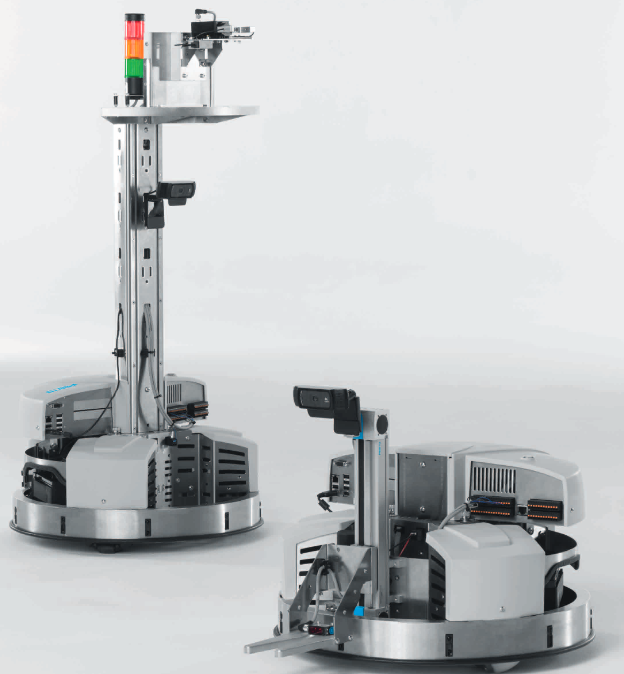
\includegraphics[scale=0.3]{Figures/RobotinoFESTO_base+torre.png}\quad 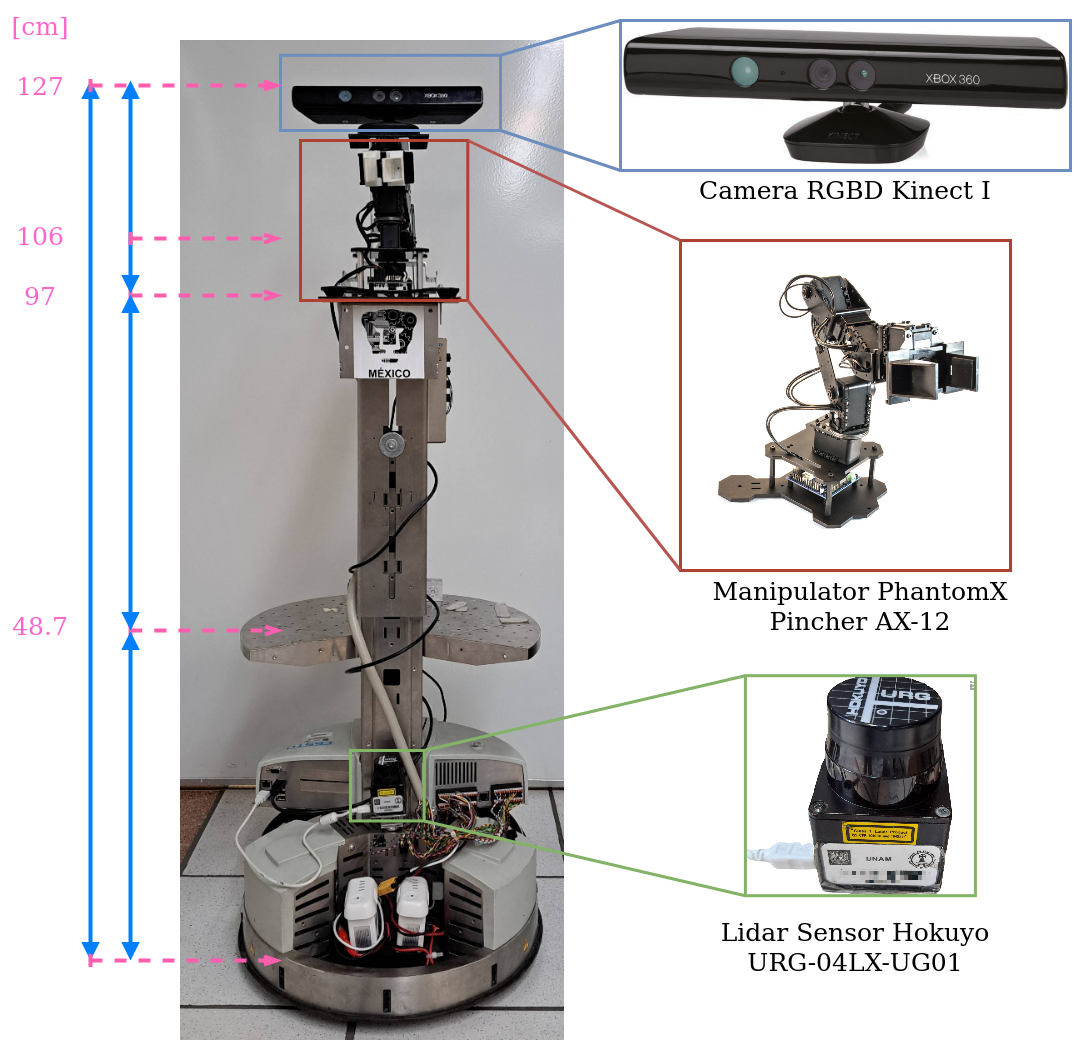
\includegraphics[scale=0.17]{Figures/Festino2023_medidas.png}                
                    \caption{Robotino 3 \cite{festo-didactic-robotino-2013} \qquad\qquad\quad\phantom{-}\qquad Robotino 3 modificado}
                    \label{fig:Robotino}
            \end{figure}
            
            %\begin{figure}[H]
            %    \centering
            %    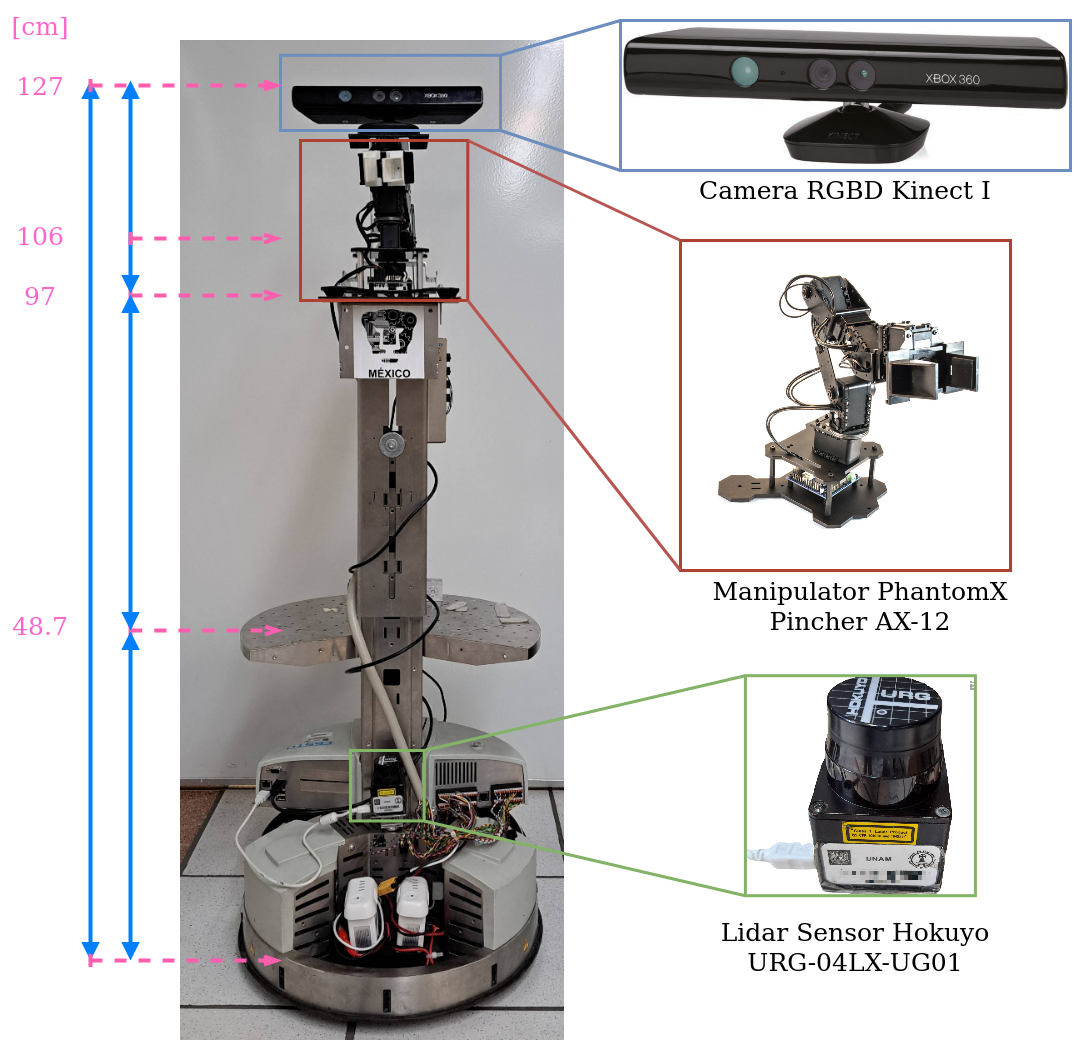
\includegraphics[scale=0.17]{Figures/Festino2023_medidas.png}
            %        \caption{Robotino 3 modificado}
            %        \label{fig:Robotino_NewNew}
            %\end{figure}
                            
            \subsubsection{Camara RGBD - Kinect}

            El autor Vangos Pterneas, ganador del reconocimiento \textit{Microsoft Most Valuable Professional (2014-2019)}, \cite{pterneas_mastering_2022} realiza una descripción del dispositivo Azure Kinect (Microsoft, 2019), así como un análisis de su impacto en la tecnología actual y las herramientas de hardware que le permiten a este aparato ser tan ampliamente utilizado, dando también una descripción de sus antecesores, los dispositivos \textit{HoloLens}, \textit{Kinect versión 2} y \textit{Kinect versión 1}.
            El autor narra que en 2009 Microsoft lanzó al mercado el dispositivo llamado \textit{Project Natal}, cambiando el nombre a \textbf{Kinect} en 2010 y distribuyéndolo como un accesorio para la consola de videojuegos \textit{XBOX 360}. Este dispositivo es capaz de reconocer las partes del cuerpo de las personas y entender sus voces en tiempo real, creando una interfaz interactiva que permitía a los usuarios utilizar la consola sin necesitar un control físico. Para el proyecto que este documento describe, se utilizó la versión 1 del Kinect, mostrado en la figura \ref{fig:Kinect_Parts}, donde también se observan los componentes del dispositivo.

            \begin{figure}[ht]
                \centering
                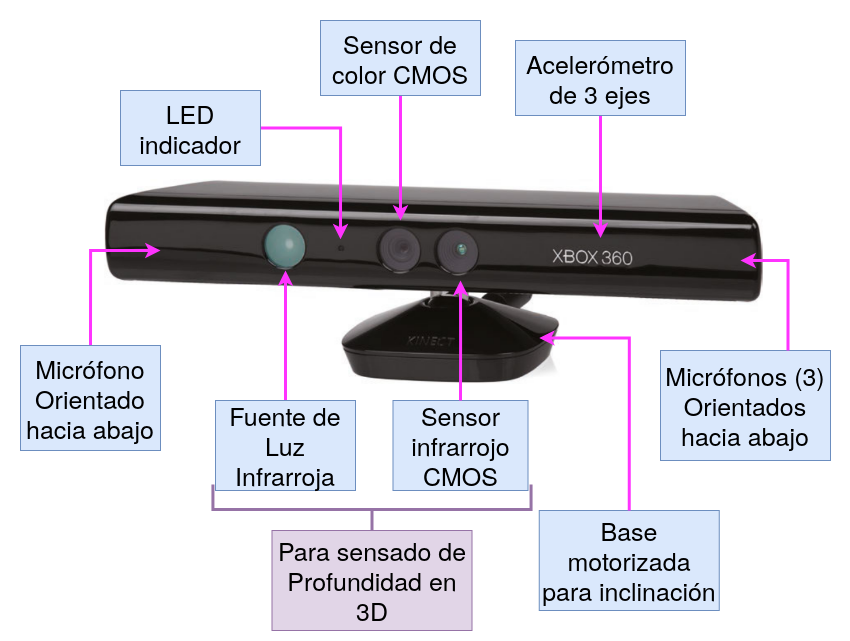
\includegraphics[scale=0.25]{Figures/Kinect_parts.png}
                \caption{Kinect versión 1 - Componentes}
                \label{fig:Kinect_Parts}
            \end{figure}

            \begin{itemize}
                \item Sensor de Profundidad \\
                En \cite{kramer_hacking_2012} Kramer et.al. especifican que el dispositivo Kinect utiliza una cámara MT9M001 (ver figura \ref{fig:Kinect_Sensors}) de la compañía Micron \cite{micron_12-inch_2004}, siendo esta una cámara monocromática con un arreglo de $1280\times1024$ píxeles, aunque estas dimensiones son modificadas antes de la reducción de resolución que se realiza posteriormente.
                Por su parte Davison, en \cite{davison_kinect_2012} describe sus especificaciones, explicando que el sensor de profundidad del Kinect consiste en una fuente de luz infrarroja que proyecta un patrón de puntos, los cuales son leídos después por un sensor infrarrojo CMOS, que detecta los segmentos reflejados del patrón de puntos, además de convertir sus intensidades a distancias. En  \cite{kramer_hacking_2012} se añade que el sensor infrarrojo crea un patrón ruidoso de luz infrarroja estructurada de 830 [nm]. El rango de profundidad del sensor tiene un alcance de 50 [cm] a 3 [m], con una resolución de alrededor de 1 [cm] sobre el eje Z, mientras que la resolución espacial (sobre los ejes X e Y) se encuentra en el orden de los milímetros. Mientras que \cite{davison_kinect_2012} también se explica que cada cuadro generado por el sensor de profundidad cuenta con una resolución de (640 $\times$ 480 píxeles), siendo capaz de mostrar 11 valores de profundidad de 11 bits, dando como resultado 2048 niveles de sensibilidad.

                \begin{figure}[ht]
                    \centering
                    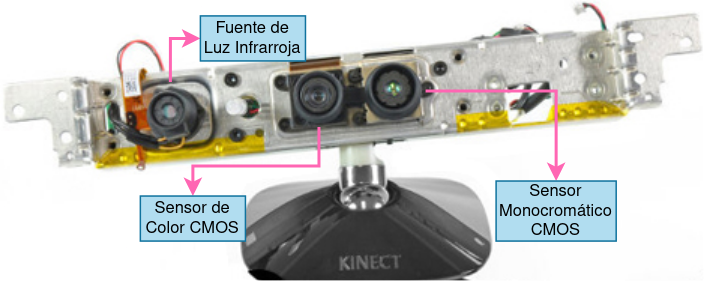
\includegraphics[scale=0.35]{Figures/Kinect_open.png}
                    \caption{Proyector Infrarrojo y Sensores CMOS \cite{eetimes_inside_2010}}
                    \label{fig:Kinect_Sensors}
                \end{figure}


            \begin{table}
                \centering
                \begin{tabular}{|c|c|}
                \hline
                \multicolumn{2}{|c|}{\textbf{Nube de Puntos}} \\
                \hline
                    Rango de Profundidad & 0.8 [m] a 3.5 [m]\\
                \hline
                    Resolución de la nube de puntos & 640 $\times$ 480 píxeles\\
                \hline
                    Niveles de profundidad & 2048\\
                \hline
                    Frecuencia de salida - Nube de puntos & 30 [Hz] \\
                \hline
                    Campo de visión horizontal & 58 \textdegree \\
                \hline
                    Campo de visión vertical & 45 \textdegree \\
                \hline
                    Campo de visión diagonal & 70 \textdegree \\
                \hline
                    Campo de visión horizontal & 58 \textdegree \\
                \hline
                \multicolumn{2}{|c|}{\textbf{Cámara RGB}} \\
                \hline
                \multicolumn{2}{|c|}{Modo \textit{Low Resolution}} \\
                \hline
                    Frecuencia de publicación & 30 [Hz] \\
                \hline
                    Resolución de Imagen & $640\times512$ \\
                \hline
                \multicolumn{2}{|c|}{Modo \textit{High Resolution}} \\
                \hline
                    Frecuencia de publicación & 15 [Hz] \\
                \hline
                    Resolución de Imagen & $1280\times1024$ \\
                \hline
                \multicolumn{2}{|c|}{\textbf{Micrófonos (4)}} \\
                \hline
                    Resolución  & 16 bits\\
                \hline
                    Frecuencia de muestreo & 16 [KHz]\\
                \hline
                
                \hline
                \end{tabular}
                \caption{Especificaciones - Kinect V1}
                \label{tab:Kinect_especs}
            \end{table}

            \item Cámara de video RGB \\
            De acuerdo con Kramer et.al (2012) \cite{kramer_hacking_2012} el dispositivo Kinect contiene una cámara RGB que, según Bob Widenhofer en \cite{eetimes_inside_2010}, utiliza un sensor MT9M112 (ver figura \ref{fig:Kinect_Sensors}). Kramer y su equipo especifican que la cámara opera a 30 [Hz] enviando imágenes de $640\times512$ píxeles. Sin embargo, es posible utilizar una configuración \textit{High Resolution}, que opera a una frecuencia de 15 cuadros por segundo, con imágenes de $1280\times1024$ píxeles. Los autore mencionan también que la cámara cuenta con balance de blancos automático, prevención de parpadeo, saturación de color, referencia de negros y correción de defectos. Los autores también resaltan que ninguno de los dos dispositivos anteriores es de verdadesa utilizad a menos de que se encuentren correctamente calibrados. 
            \end{itemize}
            
            \subsubsection{Manipulador PhantomX Pincher AX-12}
            El manipulador utilizado para este proyecto es el brazo robótico \textbf{PhantomX Pincher AX-12} distribuido por la empresa \textit{Trossen Robotics (Interbotix)}, conocida por poner a disposición del público hardware y software \textit{open source} utilizado en robótica para uso educativo, profesional o de entretenimiento. Los dispositivos de Interbotix se encuentran construidos con servomotores DYNAMIXEL X-Series, y se pueden obtener en configuraciones de 4, 5 o 6 grados de libertad, y es posible controlarlos mediante el Middleware ROS \cite{Interbotix_interbotix}. 
            
            De acuerdo con la información del fabricante \cite{Interbotix_widowx_PincherArm}, este dispositivo es un brazo robótico de 4 grados de libertad, diseñado para se compatible con la plataforma robótica \textit{TurtleBot} de ROS y cuenta con los elementos necesarios para usarlo ya sea como un elemento independiente o bien, como en este caso, integrarlo dentro de otra plataforma robótica, en la figura \ref{fig:Phantom_Pincher} se muestra un ejemplo del manipulador.\newpage
            
            \textbf{Características}
            \begin{itemize}
                \item Actuadores Dynamixel AX-12A 
                \item Base sólida con rodamiento de agujas. Construcción resistente en Delrin/acrílico.
                \item Controlador robótico Arbotix para procesamiento integrado
                \item Pinza paralela personalizable
                \item Soportes de montaje para cámaras y sensores
            \end{itemize}
            
            \phantom{saltodelineaforzado >:D}\\
            
            \textbf{Especificaciones}
            \begin{itemize}
                \item Peso: 550 [g]
                \item Alcance Vertical: 35 [cm]
                \item Alcance Horizontal: 31 [cm]
                \item Fuerza:
                \begin{itemize}
                    \item 25[cm]/ 40[g]
                    \item 20[cm]/ 70[g]
                    \item 15[cm]/ 100[g]
                \end{itemize}
                \item Fuerza de agarre de la pinza: 500 [g]
                \item Fuerza de levantamiento de la muñeca: 250[g]
            \end{itemize}

            \begin{figure}[H]
                \centering
                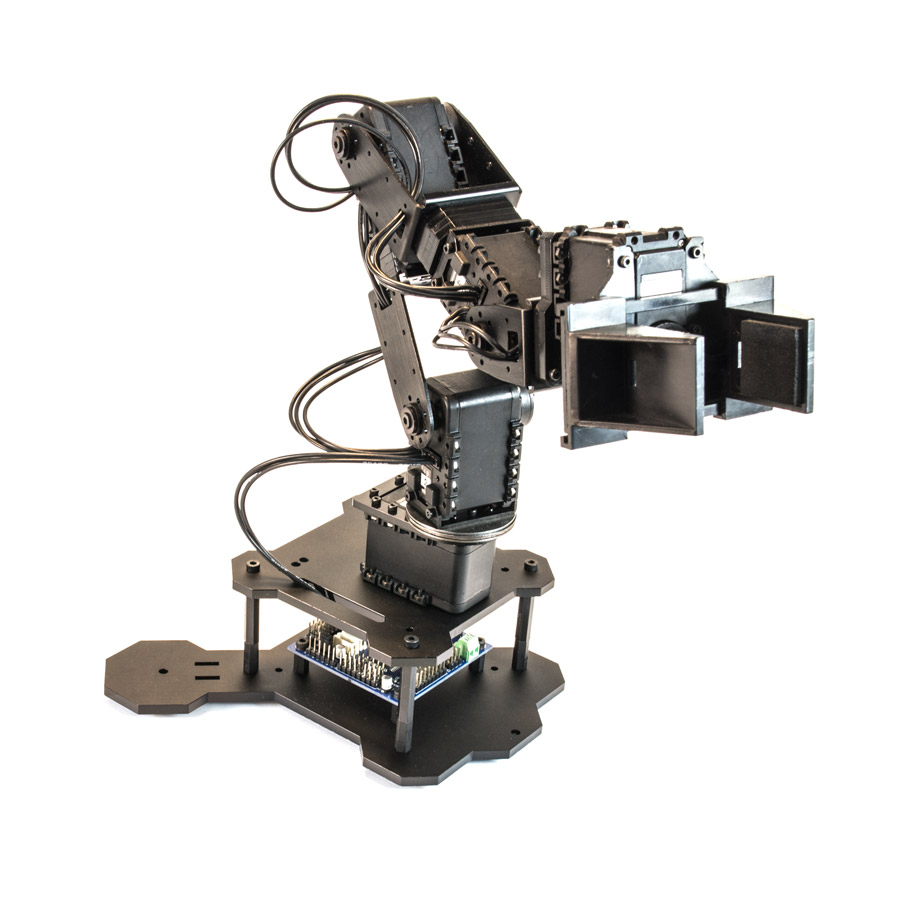
\includegraphics[scale=0.2]{Figures/Phantom_Pincher.jpg}
                    \caption{PhantomX Pincher AX-12 \cite{Inerbotix_pincher_arm}}
                    \label{fig:Phantom_Pincher}
            \end{figure}

\section{Implementación}
Para lograr la integración de todos los elementos anteriormente mencionados, los algoritmos en los que se procesa la imagen se realizan utilizando scripts de python, mientras que las máquinas de estados se programaron en C++.

La evaluación del resultado de esta implementación se dio parcialmente durante la competencia RoboCup 2023, donde se cuenta con las estaciones de trabajo y el set de piezas completas. Durante esta evaluación bajo condiciones reales fue posible observar debilidades en la implementación que fueron cubiertas posteriormente, la evaluación se continuó entonces en las instalaciones del laboratorio de Biorobótica. 

Como se ha mencionado anteriormente, se obtuvieron las medias de color de las piezas bajo diferentes condiciones de iluminación. En la figura \ref{fig:AllMeans} se muestran los colores correspondientes a dichas medias, almacenadas en un archivo yaml desde el cual el segmentador accede una vez habiéndosele indicado qué color de pieza se requiere. 

\begin{figure}[ht]
    \centering
    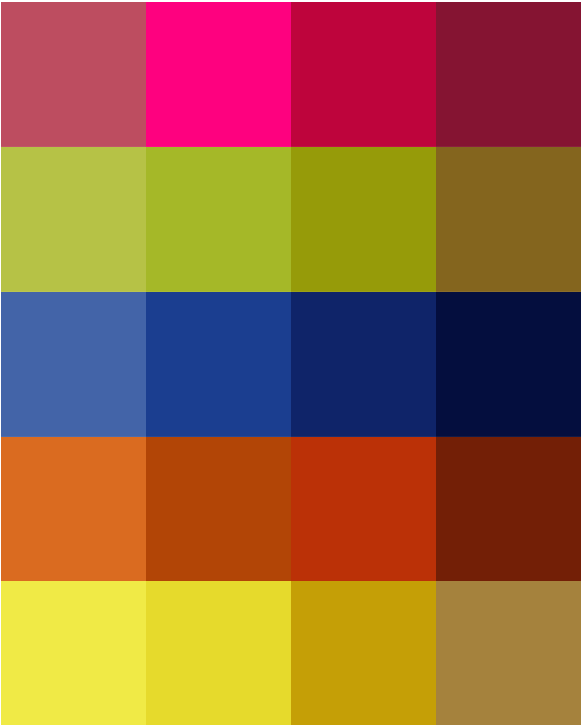
\includegraphics[scale=0.3]{Figures/AllMeans.png}
        \caption{Medias de color}
        \label{fig:AllMeans}
\end{figure}

Durante las pruebas realizadas, se observó que existe la posibilidad de confusión entre las piezas amarilla y verde. Esta confusión se asocia la cercanía de los colores en el mapa de colores correspondiente al espacio HSV usado por OpenCV. Es notable la poca diferencia entre el valor \textit{Hue} de ambas piezas (ver figura \ref{fig:ColorMapHSVOpenCV}) 

\begin{figure}[H]
    \centering
    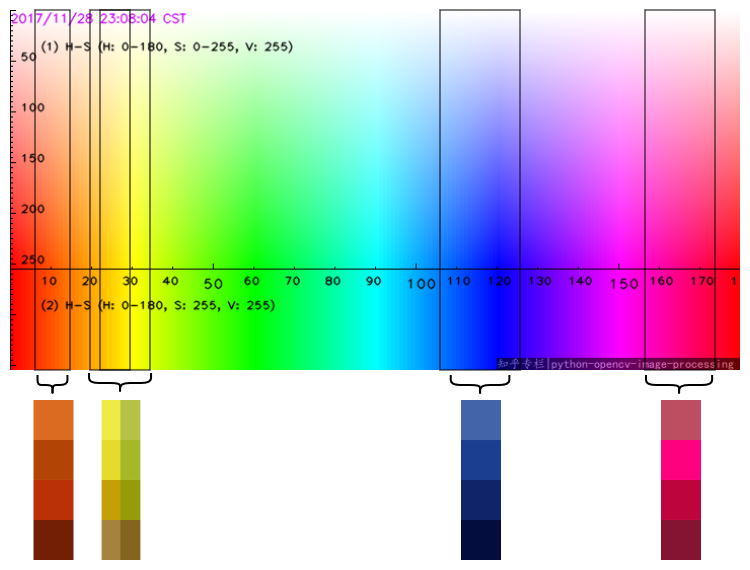
\includegraphics[scale=0.4]{Figures/PieceColors_HSVColorMap.png}
        \caption{OpenCV - Espacio HSV - Mapa de color \cite{pai_adityapai2398colour-segmentation--opencv_2022}}
        \label{fig:ColorMapHSVOpenCV}
\end{figure}

De acuerdo a la figura y a los valores obtenidos de las medias, existe un traslape entre las zonas que describen las características de color de ambos colores, mientras que para los demás elementos de interés, los cambios de magnitud son notablemente mayores. Para controlar este factor se utilizó un elemento \textit{delta} dentro de la segmentación, afectando los umbrales de los valores HSV.

\begin{figure}[ht]
    \centering
    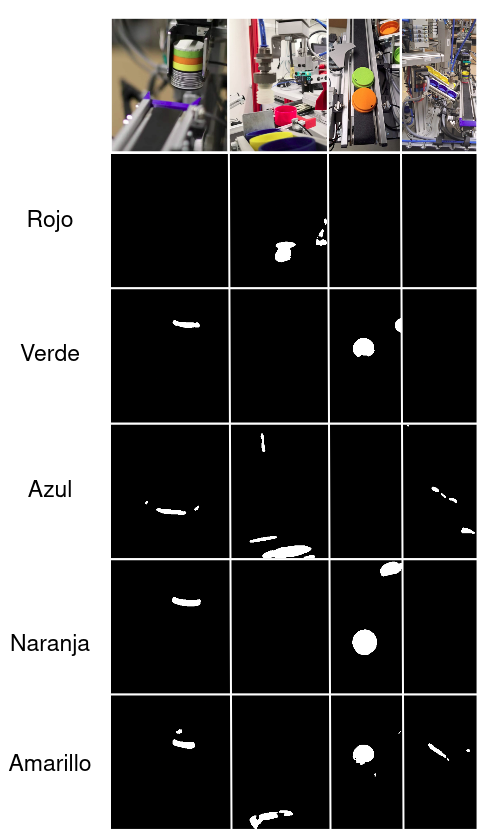
\includegraphics[scale=0.4]{Figures/AllSegmented_AllPieces_Names.png}
        \caption{Piezas segmentadas}
        \label{fig:All_Segmented_AllPieces}
\end{figure}

De esta manera, al obtener los pixeles de la imagen que pertenecen al objeto de interés, se realiza un promedio de los mismos, mediante el cual se obtiene la coordenada promedio de la posición del objeto respecto a la cámara y realizando transformaciones homogéneas se obtiene su posición respecto a la base del manipulador del robot, luego de lo cual se solicita al planeador de movimientos la trayectoria a realizar para lograr el graspeo.

Como se mencinó anteriormente, el planeador de trayectoria obtiene las posiciones angulares que de deben ser alcanzadas por los motores para lograr la posición deseada. De esta forma se establece como objetivo la coordeada correspondente al centroide de la pieza, el robot abre la pinza y realiza el movimiento de graspeo. Al encontrarse en la posición deseada, se cierra la pinza y se regresa a la posición de descanso del robot, desde la cual le es posible navegar al punto en que debe entregar la pieza nuevamente.

La evaluación del algoritmo se realizó utilizando el flujo de video obtenido de la cámara Kinect, conectado al robot y mostrando las coordenadas de los objetos buscados. En estas pruebas el objeto de interés se encontraba a una distancia horizontal mínima de 40 [cm] respecto al eje del kinect, esto debido a las limitaciones de la nube de puntos de la cámara. el experimento se realizó en 35 repeticiones, variando las posiciones de las piezas dentro del espacio de trabajo, así como la posición del robot respecto al mismo. Adicionalmente, se colocaba más de un elemento de interés en el rango visual del robot. Después de las modificaciones realizadas al parámetro delta del segmentador, el comportamiento en que se confundían piezas amarillas con piezas verdes no volvió a presentarse.

\begin{table}
    \centering
    \begin{tabular}{|c|c|c|}
    \hline
        \textbf{Pieza} & \textbf{Experimentos exitosos} & \textbf{Porcentaje de detección}\\
    \hline
        Azul & 29 & 82.85\\
    \hline
        Amarillo & 26 & 74.28\\
    \hline
        Naranja & 27 & 77.14 \\
    \hline
        Rojo & 30 & 85.71 \\
    \hline
        Verde & 29 & 82.85 \\
    \hline
    \end{tabular}
    \caption{Resultados - Detección de piezas}
    \label{tab:Res-Vis}
\end{table}

\newpage

\subsection{Resultados - Manipulación}
De acuerdo a lo establecido anteriormente, la planeación de la estrategia de movimientos se lleva acabo a través de la paquetería MoveIt, para la cual existen ya herramientas para el uso del manipulador, dentro de lo cual se cuenta con la información de la configuración mecánica el robot y sus características físicas, con dicha información se realiza la planeación de las trayectorias. Durante el proceso de prueba se observó que el manipulador puee permanecer en posición extendida cierto periodo de tiempo antes de que el motor en la primera articulación ceda ante en peso de la estructura, por lo que se definió una posición predeterminada de reposo en la cual el mecanismo del manipulador no se ve forzado \ref{fig:Arm_ResPos}.

\begin{figure}[H]
    \centering
    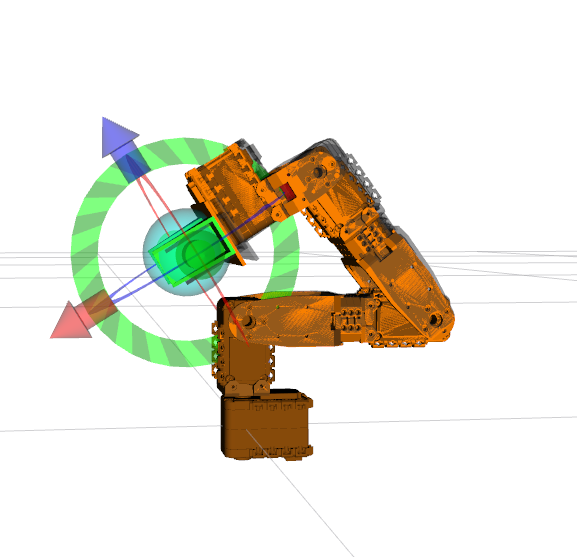
\includegraphics[scale=0.25]{Figures/Arm_RestPos.png}
        \caption{Manipulador en posición de Reposo}
        \label{fig:Arm_ResPos}
\end{figure}

Una vez que se cuenta con las coordenadas que el proceso de visión ha encontrado de las piezas de interés respecto a la imagen, se realiza la transformación homogénea para encontrar las correspondientes teniendo el origen del manipulador como referente. Estas coordenadas son enviadas a MoveIt y, después de planear la trayectoria, se realiza el movimiento. Las estrategias propuestas por MoveIt pueden variar dependiendo de la posición inicial en que se encuentre el manipulador. Sin embargo, dadas las condiciones en las que se encuentran las piezas de interés en el entorno planteado, las coordenadas en las cuales se tendría la mayor variación son $x$ e $y$, ya que la altura es constante respecto a las estaciones de trabajo. 

Para la integración de este comportamiento en la estructura general, se creó un servicio de ROS, mediante el cual los movimientos del brazo pueden ser accesados únicamente en el momento en que la máquina de estados lo solicita. Al servicio se le ingresa la coordenada de la pieza respecto a la base y una variable de confirmación del movimiento se recibe como resultado. 

\begin{figure}[H]
    \centering
    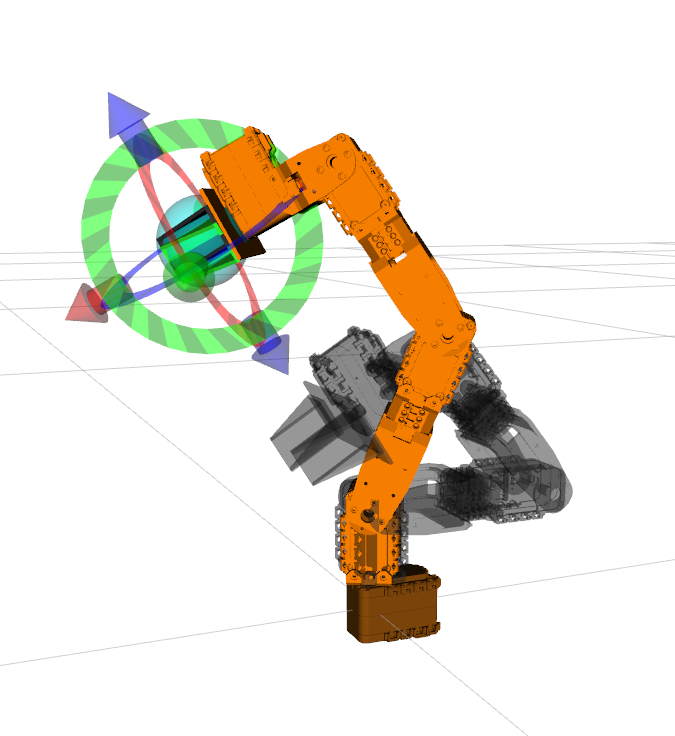
\includegraphics[scale=0.2]{Figures/Arm_MovPlan.png}
        \caption{Planeación de movimientos}
        \label{fig:Arm_MovPlan}
\end{figure}

Una de las ventajas que ofrece el uso de este manipulador se encuentra en la versatilidad de las posiciones que alcanza, pudiendo resisitir cambios en los 3 componentes de las coordenadas sin modificar la posición de la base del robot y utilizando los actuadores disponibles en su estructura, lo que lo haría capaz no solo de manipular los objetos que se encuentren en el centro de la banda transportadora, sino en cualquier otra superficie alcanzable de las estaciones, como pueden ser las plataformas de entrega y las rampas en las cuales se deshechan los elementos que no son de interés para la operación. 

La secuencia de movimientos propuesta para la tarea que se describe consiste en cuatro pasos, sin contar el inicio y vuelta a la posición de reposo. Que fueron planteados debido a las limitaciones con las que cuenta el manipulador. Esta limitación consiste en que para ciertas posiciones de $x$ o $y$, el manipulador debe comenzar desde una coordenada mínima $z = 0.12$. Adicionalmente, para el accionamiento de la pinza, es necesario bloquear los movimientos del manipulador y enviar una variable booleana, $True$ para abrir y $False$ para cerrar.

A continuación se describe la secuencia utilizada, que puede ser observada también en la figura \ref{fig:All_Segmented_AllPieces}.



\textbf{Pasos preestablecidos}
\begin{itemize}
    \item Reposo:
    \begin{multline*}
        \phantom{holis}\\
        arm\_srv.request.manipBlocker = false\\
        arm\_srv.request.x = 0.025\\
        arm\_srv.request.y = 0.0\\
        arm\_srv.request.z = 0.10\\
        arm\_srv.request.gripperState = false\\
    \end{multline*}
    \item Pinza abierta:
    \begin{multline*}
        \phantom{holis}\\
        arm\_srv.request.manipBlocker = true\\
        arm\_srv.request.x = 0.025\\
        arm\_srv.request.y = 0.0\\
        arm\_srv.request.z = 0.10\\
        arm\_srv.request.gripperState = true\\
    \end{multline*}
    \item Inicial:
    \begin{multline*}
        \phantom{holis}\\
        arm\_srv.request.manipBlocker = false\\
        arm\_srv.request.x = 0.04\\
        arm\_srv.request.y = 0.0\\
        arm\_srv.request.z = 0.12\\
        arm\_srv.request.gripperState = false\\
    \end{multline*}

    \item Trayectoria de Graspeo:
    \begin{multline*}
        \phantom{holis}\\
        arm\_srv.request.manipBlocker = false\\
        arm\_srv.request.x = det_piece.pose.position.x\\
        arm\_srv.request.y = det_piece.pose.position.y\\
        arm\_srv.request.z = det_piece.pose.position.z\\
        arm\_srv.request.gripperState = true\\
    \end{multline*}
    
    \item Pinza cerrada
    \begin{multline*}
        \phantom{holis}\\
        arm\_srv.request.manipBlocker = true\\
        arm\_srv.request.x = det_piece.pose.position.x\\
        arm\_srv.request.y = det_piece.pose.position.y\\
        arm\_srv.request.z = det_piece.pose.position.z\\
        arm\_srv.request.gripperState = true\\
    \end{multline*}
    
    \item Reposo
    \begin{multline*}
        \phantom{holis}\\
        arm\_srv.request.manipBlocker = false\\
        arm\_srv.request.x = 0.025\\
        arm\_srv.request.y = 0.0\\
        arm\_srv.request.z = 0.10\\
        arm\_srv.request.gripperState = false\\
    \end{multline*}
\end{itemize}

\begin{figure}[H]
    \centering
    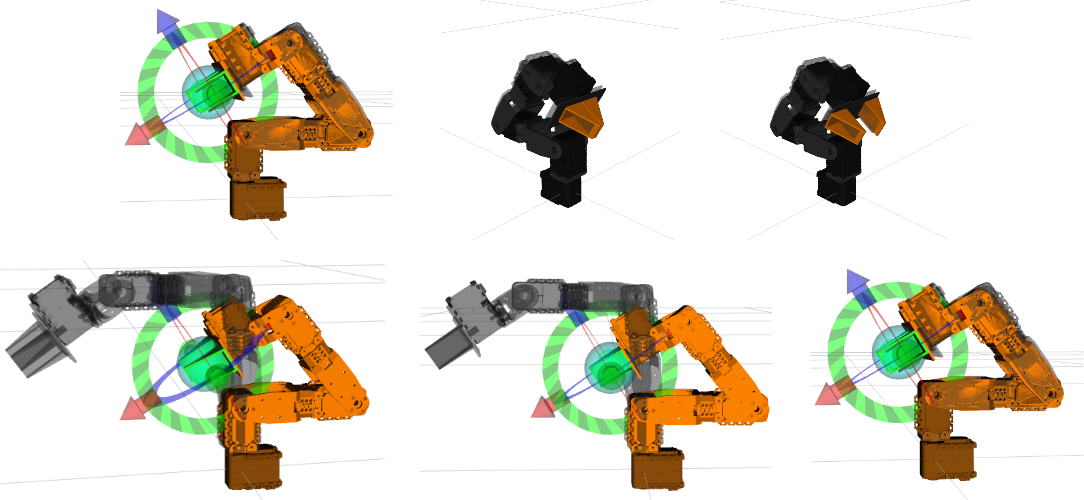
\includegraphics[scale=0.3]{Figures/Grasping_sequence.png}
        \caption{Secuencia de Graspeo}
        \label{fig:Grasping_Sequence}
\end{figure}

Debido a que en la posición de reposo la pinza obstruye la cámara del dispositivo Kinect, fue necesario determinar una posición del brazo desde la cual no interfiriera en la detección de los objetos. Para lo anterior se especificaron las posiciones angulares que debe tener cada uno de los actuadores del brazo. 


\textbf{Posición \textit{Kinect\_hide}}
    \begin{multline*}
        \phantom{holis}\\
        group.setPlanningTime(4.0);\\
        group.setJointValueTarget("arm\_shoulder_pan_joint", 2.40);\\
        group.setJointValueTarget("arm\_shoulder_lift_joint", 1.32);\\
        group.setJointValueTarget("arm\_elbow_flex_joint", 0.31);\\
        group.setJointValueTarget("arm\_wrist_flex_joint", 0.61);\\
        group.asyncMove();\\
    \end{multline*}

\begin{figure}[ht]
    \centering
    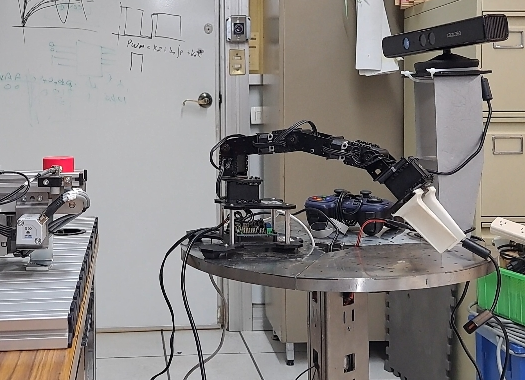
\includegraphics[scale=0.8]{Figures/Kinect_hide.png}
        \caption{Posición \textit{Kinect\_hide}}
        \label{fig:Kinect_hide}
\end{figure}

%\begin{table}
%    \centering
%    \begin{tabular}{|c|c|c|}
%    \hline
%        \textbf{Pieza} & \textbf{Experimentos exitosos} & \textbf{Porcentaje de éxito}\\
%    \hline
%        Azul & 29 & 82.85\\
%    \hline
%        Amarillo & 26 & 74.28\\
%    \hline
%        Naranja & 27 & 77.14 \\
%    \hline
%        Rojo & 30 & 85.71 \\
%    \hline
%        Verde & 29 & 82.85 \\
%    \hline
%    \end{tabular}
%    \caption{Resultados - Manipulación de piezas}
%    \label{tab:Res-Man}
%\end{table}

\subsection{Resultados - Integración}
Al proceder con la integración fue necesario hacer la unión de los modelos del robot y del brazo para poder operarse simultáneamente y que ambas partes se reconozcan una a la otra y puedan interactuar entre sí. Para lo cual se hizo una combinación de los archivos que los describen, una vez que el modelo es correcto y coincide en posiciones y orientaciones con las condiciones reales del robot se procedió a probar los algoritmos que se plantearon anteriormente. 

Anteriormente se mencionó de forma breve que al realizar estas pruebas conjuntas, y dado que en la estructura de la máquina de estados se definía que se realizarían secuencialmente los movimientos de base del robot, del manipulador y la ejecución del algoritmo de visión, se obtiene un error debido a la vibración que genera el manipulador en la estructura sobre la cual se encuentra el Kinect. 






\input{Ch07_Discusión}
\end{document}
